\documentclass[12pt, twocolumn, x11names]{article}

\usepackage{amsmath}
\usepackage[draft]{hyperref}
\usepackage{graphicx}
\usepackage{tikz}
\usepackage{booktabs}
\usepackage{caption}
\usepackage{subcaption}
\usepackage{epigraph}
\usepackage{multirow}
\captionsetup[figure]{font=small}
\captionsetup[table]{font=small}
\captionsetup[subfigure]{font=scriptsize}

\usepackage{sectsty}
\sectionfont{\bfseries \normalsize \uppercase}
\subsectionfont{\normalsize}
\subsubsectionfont{\normalsize \normalfont \itshape}


% \usepackage{multicol}
\setlength{\columnsep}{0.5cm}
\setlength{\parskip}{0pt}

\usepackage[a4paper, total={7in,8in}]{geometry}

% bibliography tings
% TODO: find a nice author-year bibstyle
\usepackage{natbib}
\bibliographystyle{ametsoc2014}
%\usepackage[maxcitenames=3, maxbibnames=3, style=ametsoc2014.bst, backend=biber, natbib=true]{biblatex}
%% \setcitestyle{authoryear}
%% \AtEveryBibitem{\clearfield{month}}
%% \AtEveryBibitem{\clearfield{day}}
%% \AtEveryBibitem{\clearfield{isbn}}
%% \AtEveryBibitem{\clearfield{issn}}
%% \AtEveryBibitem{\clearfield{doi}}
%% \AtEveryBibitem{\clearfield{url}}
%% \AtEveryBibitem{\clearfield{eprint}}


\newcommand{\elnino}[0]{\emph{El Ni\~no}}
\newcommand{\enso}[0]{\emph{ENSO}}
\newcommand{\nina}[0]{\emph{La Ni\~na}}

% TODO A better title. Something witty and fun.
\title{\elnino{} and Africa}
\author{Luke Conaboy and Mark G. Skilbeck}
\date{}

\begin{document}

\twocolumn[
  \begin{@twocolumnfalse}
    \maketitle
    \begin{abstract}
      This is driving me to abstraction
    \end{abstract}
  \end{@twocolumnfalse}
]

  \clearpage

  \vspace*{\fill}
  \setlength\epigraphwidth{.8\textwidth}
  \epigraph{\Huge I bless the rains down in Africa}{--- \emph{Africa}, Toto}

  \clearpage

\section{Introduction}

The importance of weather forecasting cannot be understated. We regularly
consult weather forecasts to inform our clothing choices, to help us decide
whether a family outing should be a trip to the beach or to a museum; should we
bring along an umbrella? is it shirt-and-shorts weather?\footnote{Incidentally
  it is never \emph{shirt-and-\textbf{short}-shorts weather.}} These are
legitimate concerns, but they are decidedly \emph{first-world} concerns. In
parts of the world where the amount of rainfall literally means life or death it
is plainly obvious that forewarning of drought is of paramount importance.
Whereas wealthy nations may import food and water in times of need, much of
sub-Saharan Africa relies on the prosperity of local agriculture to meet dietary
needs. Any negative impact on the harvest -- here we concern ourselves only with
climatological causes -- will severely restrict available food sources
\citep{development2006mapping}.

Modern Africa has been plagued by socioeconomic struggles, with frequent civil
war, little access to education and medicine, and highly unstable
governments. While much progress has been made in recent years\footnote{For more
  information see \url{https://africaindata.org}} the extra stresses of food
shortages and drought may trigger a return to instability.
% TODO Provide actual citation for above. Is the last line here a
% bit... insensitive?
In 2016 the UN Office for the Coordination of Humanitarian Affairs (UNOCHA)
published a report on the response to \elnino{} in East and Southern Africa
\citep{unocha2016}; by their estimates over 19.5 million people and 10.5
children were affected in East Africa alone. As a result of \elnino{} parts of
East Africa received below average rainfall leading to poor harvests and food
shortages. Similarly, parts of Southern Africa experienced the worst drought for
35 years and leading to huge food insecurity. As one of the worst hit countries,
Kenya alone now has over 1.2 million people in a food security crisis.

Malaria has long been a leading cause of death in Africa, particularly in
children, accounting for approximately 18\% of total deaths in children
\citep{IMHE2016}. \citet{Alles1998} states that, at the time of reporting,
malaria transmission intensities---a measure of how effectively malaria is
transmitted in a population---are often two orders of magnitude greater than other
regions where malaria is a significant problem. \citet{loevinsohn1994}
investigated the relationship between climatic warming and malaria incidence
rates in Rwanda, East Africa. The report found that during the particularly warm
period of the late 1980s malaria incidence rates almost doubled, with even
regions previously free of the disease showing an up-take in
incidence.\footnote{Interestingly, the report notes that while there was no
  significant trend in precipitation over the same period, there was heavy rain
  in the years 1987 and 1988 which coincided with a strong ENSO event.}

More recently \cite{craig2004} sought to quantify the association between
various climatic factors---including rainfall and temperature---and malaria
incidence. The report found that \emph{total seasonal cases} of malaria were not
driven by climatological factors; however there was a strong correlation between
interseasonal variability and factors such as the maximum temperatures of the
preceding season.


% For this reason, it is imperative that we improve our understand of and ability
% to predict this effect in order that we may better prepare and coordinate
% responses to prevent humanitarian disasters.

%% % Would like to say something here referencing data on drought related
%% % deaths in Africa.
%% Indeed forewarning of any impending weather is
%% important for different reasons depending on the local agriculture:
%% forecasting drought allows for stockpiling of water and foods;
%% forecasting of inclement weather allows for farmers to prepare for a
%% greater yield, and locals to prepare for possible flooding.
%% % What other reasons are there for forecasting? This needs rewriting
%% % anyway, as it is a bit ugly in terms of wording. Could be more poetic.
%% Where discussion of the weather is not ``should I wear a raincoat?''
%% but ``will we have enough drinking water?'' weather forecasting should
%% be considered a humanitarian imperative. 
% Is there something to say about global warming here? Probably.

\vspace{1cm}

Early twentieth century observations of atmosphere pressures showed a peculiar
relationship between those measurements in the western tropical Pacific and
those in the southeastern tropical Pacific \citep{holton1989}. Namely, that they
were out of phase --- when one measure was positive, the other was negative.
This was termed the \emph{Southern Oscillation}. Later studies \ref{TODO} would
show that there were accompanying variations in rainfall, sea surface
temperatures, and wind patterns. The combination of these effects would come to
be known collectively as the \elnino{} \emph{Southern Oscillation}, with the
warm phase named \elnino{} and the cold phase \nina{}.


\subsection{Southern Oscillation}
Since the late 19th century, the existence of a large scale `seesaw' in oceanic
surface pressure across the Pacific had been observed \citep{trenberth2000}. The
essence of this observation is that when air pressure is high over the Pacific
Ocean, air pressure tends to be lower over the Indian Ocean (and vice versa)
\citep{philander1990}; from this it was inferred that the two regions were
causally connected by some then-unknown meterological teleconnection. It was
Walker and Bliss who, in the 1930s, characterised this pattern using measures
% Could/should probably say in more detail how exactly they characterised this
such as sea level pressure and precipitation, naming it the Southern Oscillation
(SO). Walker also defined an index for the SO, calling it the Southern
Oscillation Index (SOI). Figure \ref{fig:slp_corr} shows the average spatial
distribution of SOI correlations for the Pacific, showing the eastern and
western Pacific to be out of phase.
% TODO Some more discussion of indices here. Describe exactly what SOI is,
% describe other indices, particularly ones we use.

\begin{figure*}
  \centering
  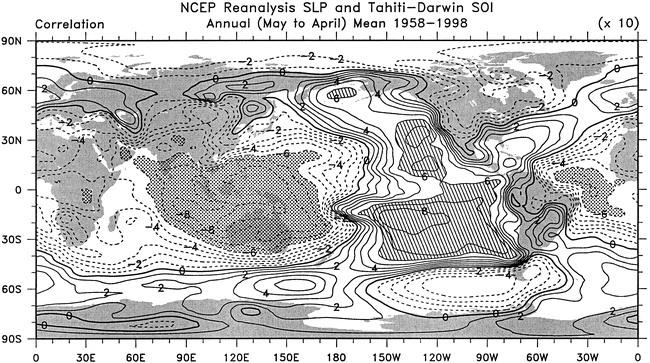
\includegraphics[width=0.75\textwidth]{figures/slp_corr}
  \caption{Sea level pressure correlations with Southern Oscillation Index, a
    measure of the SO devised by Walker. Regions with correlations $>0.6$ are
    hatched and those $<-0.6$ are dotted. It is clear to see that the eastern
    and western tropical Pacific ocean are anticorrelated. Figure taken from
    \cite{trenberth2000}.
    % TODO Is it clear? Maybe this needs more exposition.
  }
  \label{fig:slp_corr}
\end{figure*}

While Walker managed to characterise the atmospheric component of the SO, the
interannual pressure fluctations driving it were irregular and there was not
enough data for Walker to determine whether the ocean was involved in the
system.

\vspace{0.5cm}

In his seminal 1961 study Bjerknes began formulating a model of how the
interaction of both athmospheric and oceanic components could lead to the
appearance of \elnino{} conditions over the tropical Pacific
\citep{bjerknes1961}. He reasoned that much of the connection lied in weakening
of trade (east-to-west equatorial) winds owing to natural fluctuations caused,
for example, by the uneven solar radiation. The trade winds at the sea surface
drag surface water with them. When the trade winds weaken, the friction between
air and sea surface is reduced, thus allowing warmer western Pacific water to
flow to the cooler east. An abundance of warm water along equatorial South
America then surges into the Peruvian coast, as observed by the Peruvian
fishermen.

Later \citep{bjerknes1966} it was also noted that weakening of the trade winds
would lead to reduced upwelling. The general view of the tropical Pacific is of
relatively warmer waters in the west (near Australia), gradually cooling towards
the east (near Peru). This is typically described as having a thermocline (where
cold water meets warm water) gradually rising from west to east. If the trade
winds weaken the thermocline becomes depressed in the east due to the
aforementioned resurgence of warm water. The anomalous warming of seas then
imparts energy into the atmosphere above. Bjerknes states in his conclusion:
``So much seems certain, however, that the extensive warmings of the East
Pacific equatorial waters are due to a weakening of the equatorial easterly
winds to such an extent that (a) the normal upwelling appreciably weakens of
even ceases'', making the case for an ocean-atmosphere connection.

A key result of \citep{bjerknes1966} is that by using the above reasoning
Bjerknes was able to link strengthening of westerlies in the middle latitudes
occuring with accompanying warming of equatorial ocean water. Bjerknes reasoned
that anomalous warming of surface water would then increase the \emph{Hadley
  circulation} rate, thus leading to increased westerly wind strengths.

The Hadley circulation is the poleward atmospheric circulation of
equatorial air away from the equator. The process is diagrammed in
\ref{fig:hadleycell} and is as follows \citep{geomar6557}. Warm air carried by
the trade winds (moving in an easterly and equatorial direction) converges at
the equator where it releases moisture and rises. The Earth's rotation causes a
Coriolis force which results in the rising air being pushed poleward. The
Coriolis force is clockwise in the Northern hemisphere and anti-clockwise in the
Southern hemisphere; in both cases, as the air moves poleward it also
experiences an eastward motion, whereas at the equator it is moving westward
with the trade winds. Having cooled, the air begins to sink at the upper
latitudes, where the Coriolis force now brings the air back towards the equator,
eventually with an easterly component --- the trade winds.

\begin{figure}[t]
  \centering 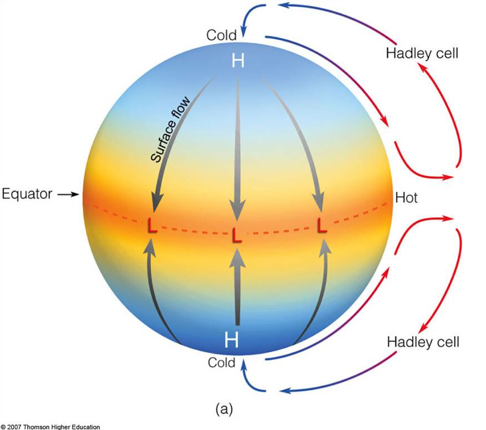
\includegraphics[width=0.9\linewidth]{figures/hadleycell.png}
  \caption{The Hadley circulation. Warm air rises at the equator, is pulled away
    from the equator and towards the poles, cools and falls at greater
    latitudes, then is pulled back towards the equator. This circulation is
    largely created by uneven solar heating and the Coriolis force due to the
    Earth's rotation.}
  \label{fig:hadleycell}
  % From https://www.seas.harvard.edu/climate/eli/research/equable/hadley.html
\end{figure}

Bjerknes continued his investigation into the causes and effects of anomalous
heating in the tropical Pacific ocean and atmospheric pressure variation in his
1969 study \emph{Atmospheric Teleconnections from the Equatorial Pacific}
\citet{bjerknes1969}. In this study a clear connection between \elnino{} and the
SO was demonstrated, particularly that a 1963 \elnino{} event caused a strong
response in the SO.

Figure \ref{fig:pressureprofiles} shows how the dynamic height of a number of
isobars (surfaces of constant atmospheric pressure) varies along the equator
during the months January 1960, and July 1960. In both months it can be seen
that, in the region marking the Pacific ocean, the streamline gradient closest
to the sea surface is towards the west (indicated in \ref{fig:pressureprofiles}
by the line ``S.L.''). Since the streamline gradient shows us how air would move
subject to atmospheric pressure, we can infer that air at that height is moving
east-to-west. As that air moves westward, the sea surface is warming and so the
air warms also, rising as it does. Next we see that at greater heights (in
Figure \ref{fig:pressureprofiles}, lines ``300'' to ``150'', the gradient of the
streamlines is reversed, and we have west-to-east motion along these
streamlines. Progressing eastward and cooling, the air begins to fall,
eventually completing one cycle of what Bjerknes labelled the \emph{Walker
  Circulation}.

\begin{figure}[t]
  \centering
  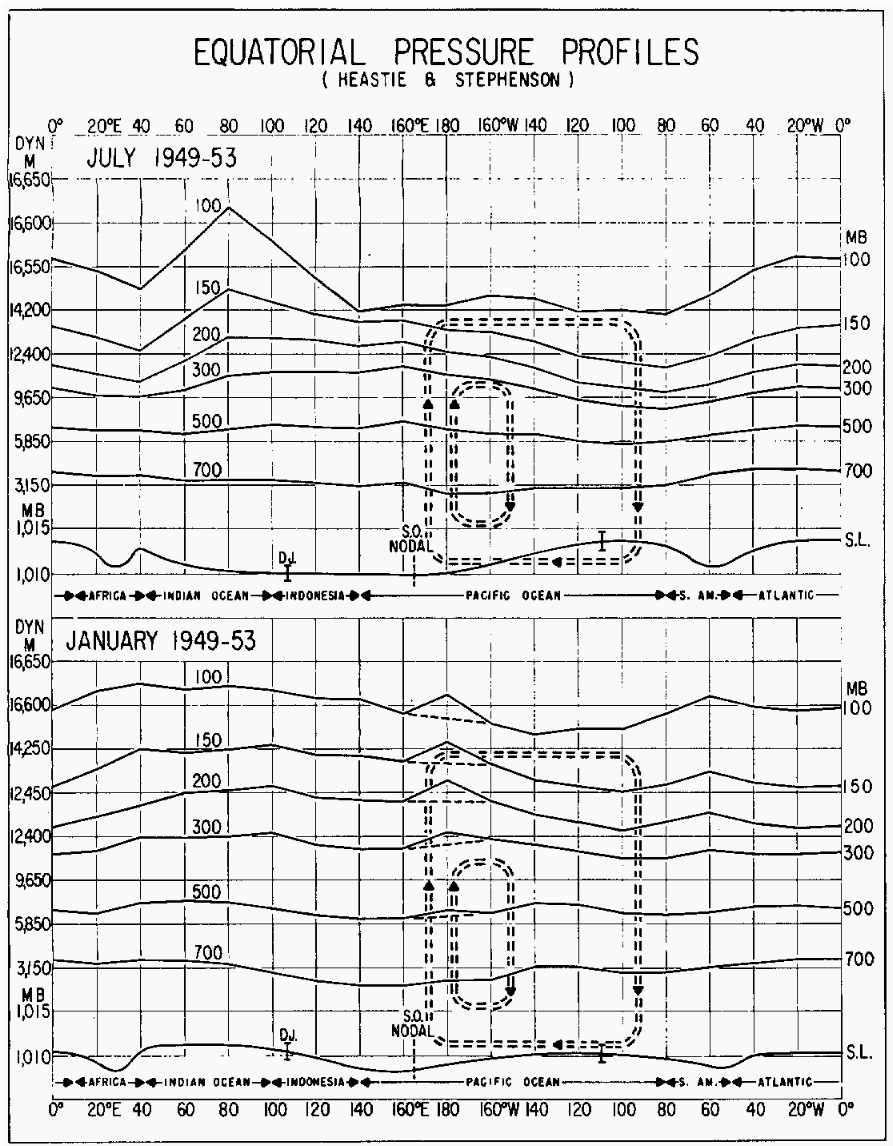
\includegraphics[width=0.9\linewidth]{figures/equatorial-pressure-profiles.png}
  \caption{Height of isobaric streamlines along equator. The \emph{Walker
      circulation} is shown over the Pacific ocean in double-dashed lines, with
    direction indicated by arrows. Source: \citet{bjerknes1969}}
  \label{fig:pressureprofiles}
\end{figure}

Bjerknes states that ``The Walker Circulation ... must be part of the mechanism
of the still larger ``Southern Oscillation'' ...''.

% Diagram here.

%% \cite{bjerknes1969} proposed the currently accepted model for
%% atmospheric circulation driving the SO, calling it the Walker circulation. In
%% this model, dry air sinks over the cool water of the eastern tropical
%% Pacific. After sinking it is transported westward along the equator by the
%% easterly trade winds. As it travels over progressively warmer water the air is
%% warmed and moistened, until it finally reaches the western tropical
%% Pacific. Here the air is now very warm and saturated with water, and it rises in
%% prodigious rain clouds. The circulation is completed with the return flow of air
%% through the upper trophosphere.

%%  % TODO Definitely need some figures here for the Walker circulation.

%% This atmospheric circulation also drives oceanic currents. Water is driven east
%% to west, warming as it goes. This allows for cooler water to rise from the
%% depths along the eastern Pacific, a process called \emph{upwelling}. Combining
%% the oceanic and atmospheric circulations in the Pacific yields a potential
%% explanation for the \elnino\ phenomenon.

\subsection{\elnino-Southern Oscillation}
The Walker circulation requires an east-west tropical Pacific SST gradient for
the transportation of air. An initial positive SST anomaly in the eastern
Pacific ocean would diminish the east-west gradient. A diminished SST gradient
reduces the Walker circulation, in turn weakening the westerly equatorial trade
winds \citep{lindzen1987}. Warm water that was previously being driven westward
by the trade winds can now flow back toward the east, preventing upwelling and
reinforcing the intitial SST anomaly. Through positive feedback between the
ocean and the atmosphere, an initial SST anomaly can lead the equatorial Pacfic
into a warm state -- \elnino. Since the pheneomenon is due to ocean-atmosphere
interaction, the whole system is termed the \elnino-Southern Oscillation
(ENSO). {}\nina\ corresponds to the cold state of ENSO, characterised by
negative SST anomalies and keen trade winds.

%% oscillatory, modes, period

\subsection{Teleconnections}
%take about what drives the teleconnections, i.e. changing circulation
ENSO affects not only the climate of the local Pacific region, but can extend
farther out to influence regions of Africa and Europe \citep{moron1998}. The
magnitude of the influence in these places is weak, but present
nevertheless. Multiple comprehensive studies \citep{ropelewski1987,
  ropelewski1989, nicholson1996} have found that ENSO modulates the rainfall of
continental Africa, although there is some dispute about regional impact
\citep{wolter1989}. Figure \ref{fig:enso_rainfall_anoms} shows the latest
comprehensive study of seasonal rainfall anomalies for ENSO events.

\begin{figure*}
  \centering
  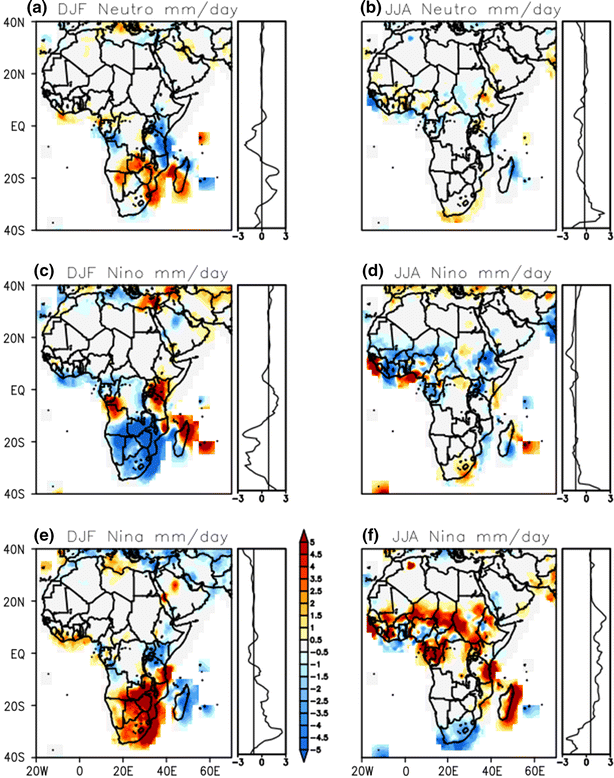
\includegraphics[width=0.7\textwidth]{figures/enso_africa_rainfall_anoms}
  \caption{Distribution of precipitation anomalies and latitudinal averages in
    mm/day, for the DJF and JJA seasons. Panels a) \& b) show neutral years, c)
    \& d) show \elnino\ years and e) \& f) show \nina\ years. The distributions
    show that southern and equatorial Africa exhibit the strongest responses to
    ENSO events, in the DJF and JJA seaons, respectively. DJF corresponds to the
    rainy season and JJA to the dry season for southern Africa and the opposite
    is true for equatorial Africa. Figure taken from \cite{deoliveira2018}.}
  \label{fig:enso_rainfall_anoms}
\end{figure*}

\subsection{Indian Ocean}
On interannual timescales, ENSO is the predominant form of climate variation
\citep{obrien1998}, however it is not the only system that can affect weather on
the African continent. An ocean-atmosphere mode in the Indian Ocean, caused by
anomalously high (low) sea surface temperatures in the western (eastern) regions
of the ocean, was identified by \cite{saji1999} and is starting to be considered
as an influential player in climate dynamics. \cite{anyamba2002} suggest that
the observed vegetation response in regions of Africa between $1997-2000$ was
more significantly driven by these western Indian Ocean SST anomalies, than
anomalies in the Pacific. This mode, called the Indian Ocean Dipole (IOD) has
also been linked to the `Big Dry' -- the severe drought that has been ongoing in
southern Australia since 1995 \citep{karumuri2003, ummenhofer2009}.

Furthermore, the effects of the IOD are not solely continental -- there is
evidence to suggest that the IOD can be involved with the ENSO itself. There
have been multiple studies into its role as a contributor to both the growth
\citep{annamalai2005, hackert2017} and demise \citep{okumura2010, kug2006,
  xie2009, dayan2015} of \elnino{} events. \cite{dong2018} propose that not only
can the IOD influence an established \elnino{} event, but that it may in fact be
able to stop an \elnino{} event developing at all. It follows, then, that in
order to better predict \elnino{} events we must take the Indian Ocean into
account \citep{hackert2017}.

\subsection{Cloud Coverage}
\label{sec:intro:cc}

Fill this out using literature reviews, etc.

\subsection{Normalised Difference Vegetation Index}
\label{sec:intro:ndvi}

Use \cite{yengoh2014}, \cite{bannari1995}, and lit reviews.


% mark you know more about NDVI and calibration so you may want to flesh this
% section out e.g. calibrations
Green vegetation has a distinctive spectral response to electromagnetic
radiation. Radiation in the near-infrared is reflected while the chlorophyll in
leaves absorbs strongly in the red. Hence we determine vegetation coverage using
the normalised difference vegetation index (NDVI) defined as

%% Local Variables:
%% fill-column: 80
%% End:

\section{Data}

Here we should include a short section describing the data we have,
where we got it from and any interesting things to do with it.

\section{Method}
In this section we discuss the way in which we process and analyse the data we
obtain from EUMETSAT. First we detail the process of thresholding, which we use
to distinguish between cloud and land pixels. Then, we explain how these
thresholds are used to create useful data products from the raw data.

\subsection{Thresholding}
\label{sec:method:thr}
The most essential part of processing the EUMETSAT images is the ability to
differentiate between cloud and land. Clouds have a much higher reflectance than
land (notable exceptions to this are snow, ice and salt pans) -- if mistakenly
identified as land pixels, they will erroneously skew the value of those pixels
to higher values.

On a clear day any given pixel should have a value that corresponds to that
pixel's ``true'' value (hereafter the \emph{ground} value), with some small
variation contributed by shadows cast by nearby clouds, the variation in
\emph{solar zenith angle} throughout the year, and atmospheric interference
effects. On a cloudy day a pixel's value will be systematically pulled towards
higher than ground values. It follows then that the distribution of a pixel's
value will be bimodal, with the lower peak corresponding to the ground value,
and the large peak corresponding to cloudy values.

The task is then one of producing thresholds that reliably separate the two
peaks. Otsu's method \citep{gonzalez2008} separates pixels into two groups, or
\emph{classes}, by maximising the variance between these classes, making it an
optimum method for thresholding\footnote{We have made use of \texttt{scipy}'s
  Otsu thresholding implementation.}. An example of Otsu thresholding at work is
shown in Figure \ref{fig:otsu} for a random pixel.
\begin{figure}
  \centering
    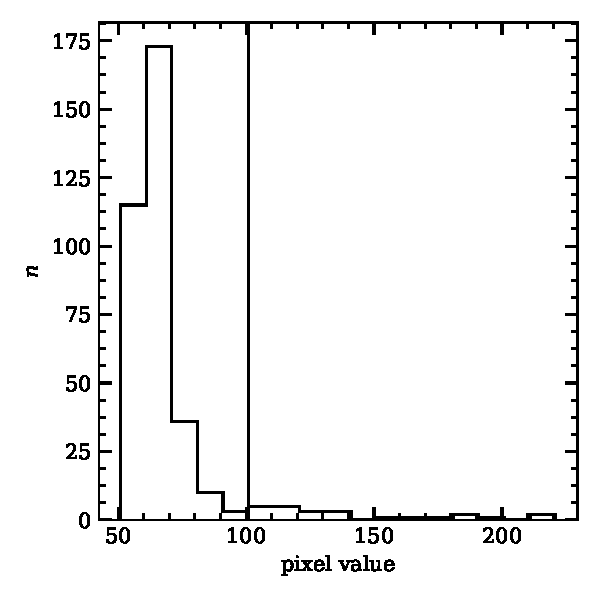
\includegraphics[width=0.8\linewidth]{figures/otsu_bimodal.pdf}
    \caption{The histogram of pixel values for a random pixel. Shown by the
      vertical line is the threshold calculated using Otsu's method -- it can be
      seen how well this method separates the two peaks.}
    \label{fig:otsu}
\end{figure}
All pixels with a value below the threshold will be identified as land and all
pixels with a value greater than or equal to the threshold will be identified as
cloud. Please refer to Section \ref{sec:disc:thresh} for a discussion of
suitable we determined Otsu's method to be in identifying cloud.

Now that we have the method for calculating the threshold of a single
pixel all that remains is to apply it to the entire image, the process for doing
so is detailed in Figure \ref{fig:thr_fc}.
\begin{figure}[t!]
  \centering
  \includegraphics{threshold_flowchart.pdf}
  \caption{Flowchart for calculating threshold values.}
  \label{fig:thr_fc}
\end{figure}

\subsection{Cloud coverage}
Using the thresholds calculated by the method in Figure \ref{fig:thr_fc} we
produce daily cloud masks, which are arrays of the same size as the input image
containing with values of 1 for cloud pixels and 0 for land pixels. The number
of cloud pixels $n_{\mathrm{cloud}}$ for a given day, then, is found by summing
the cloud mask. Cloud coverage is calculated as the ratio of cloud pixels to
total land pixels in the image $N$
\begin{equation}
  \mathrm{CF} = \frac{n_{\mathrm{cloud}}}{N} \,,
  \label{eq:cloud_frac}
\end{equation}
where $N$ is found by summing over all of the land pixels in the land mask for
the given region.

\subsection{Vegetation}

\begin{figure*}
  \centering
  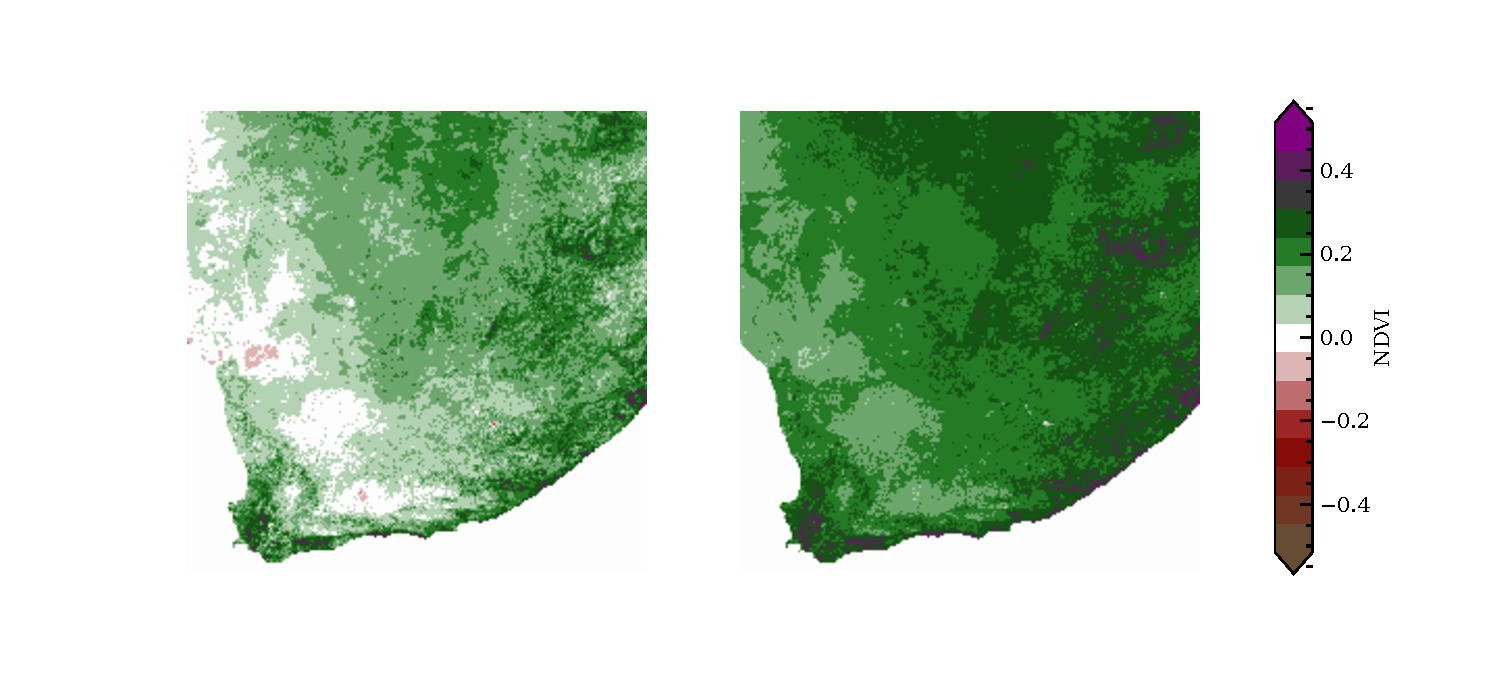
\includegraphics[width=0.85\textwidth]{figures/ndvi_calibration_comparison.pdf}
  \caption{Comparison between NDVI calculated for uncalibrated data (shon left),
    and calibrated data (shown right). The uncalibrated NDVI shows a wider range
    of values, with large areas where NDVI is close to zero (in which case
    $\rho_{\textrm{NIR}}\approx\rho_{\textrm{R}}$), and some regions where NDVI is
    negative. The calibrated NDVI shows neither of these traits, and so we can
    see how using uncalibrated NDVI would lead to erroneous conclusions.}
  \label{fig:calibrationcomp}
\end{figure*}

As described in Section \ref{sec:data:calib} the raw data in the PNG files are
\emph{pixel count} data, \emph{not} radiance data. Before any NDVI calculations
are performed we must calibrate each data channel, so that we have the radiance
data which is required for NDVI. The calibration data is listed in Table
\ref{tab:calibration}. As a matter of interest, a visual comparison of NDVI with
and without calibration is show in Figure \ref{fig:calibrationcomp}. With the
calibrations complete, Equation \eqref{eq:ndvi} is used to calculate the NDVI.

\subsection{Analysis}
In order to make useful comparisons with our data products, we need some method
of determining whether a measurement is anomalously large or small in comparison
to some baseline value. The baseline value will generally be a year-long
average, though occasionally the median is a better choice where outliers exist
in the data. 

Weather data are inherently noisy over day-to-day timescales, so first we smooth
the data by taking monthly averages. As can be seen \ref{fig:smoothcomp}, the CF
varies rapidly day-to-day and so obscures any underlying features in the
data. Smoothing that data by averaging over a larger period reduces the daily
variation, leaving the larger trends visible. 

Once we have baseline measurements, we can then calculate the anomalies which
tell us how different a particular measurement is from the average for that time
of year. If $x_{i}$ is the measurement (e.g. NDVI) for a particular month and
year then we define the anomaly as
\begin{equation}
  x_{i\sigma}=\frac{x_{i}-\tilde{x}_m}{\tilde{x}_m}
  \label{eq:anoms}
\end{equation}
where $\tilde{x}_m$ is the median value for that month. The $\tilde{x}_m$ are
defined by calculating the median for each month across the all of the available
years.

Weather patterns like the ENSO vary over a few months or longer, so we are
interested in signals of a similar timescale. To be confident that what were
observing is relevant, and not just transient, we smooth the monthly anomalies
using a five month moving average. Smoothing is done in an efficient way by
using convolution \citep{gorry1990}.

The particular choices for baselines and smoothing parameters in each of our
analyses will be described and justified in more detail in the respective
sections.


%% Local Variables:
%% fill-column: 80
%% TeX-master: "report"
%% End:

% TODO make sure quoted values are accurate (i.e. look em up)
\section{Results}
This section is split into two parts, the first looking at the results
of our cloud coverage analysis and the second looking into the NDVI
analysis.
\subsection{Cloud coverage}
\subsubsection{Rainfall}
Figure \ref{fig:cf_rf} shows the monthly averages of cloud fraction
over the period $2008-2017$ and rainfall over the period $1991-2015$
for South Africa (Figure \ref{fig:cf_rf_south}) and East Africa
(Figure \ref{fig:cf_rf_east}). For both cloud fraction and rainfall, a
sinusoidal curve with a period of $T=12$ months has been fitted to
better highlight the seasonal dependencies. From Figure
\ref{fig:cf_rf_south} we see that South Africa has the largest values
of cloud fraction and rainfall at the beginning and end of the year
(local summer), with cloud coverage of $\sim0.2-0.3$ and rainfall of
$\sim70$ mm. During the middle of the year (local winter), cloud coverage
falls below $0.1$ and rainfall drops to $\sim20$ mm. Now looking at
Figure \ref{fig:cf_rf_east} we see the opposite trend for East
Africa. Cloud coverage and rainfall are at there smallest values at
the beginning and end of the year (local winter), at $\sim0.4$ and $\sim21$
mm respectively. As we head toward the middle of the year (local summer), cloud coverage and rainfall peak at $\sim0.2-0.3$ and $24$ mm respectively.
\begin{figure}
  \begin{subfigure}{\linewidth}
    \centering
    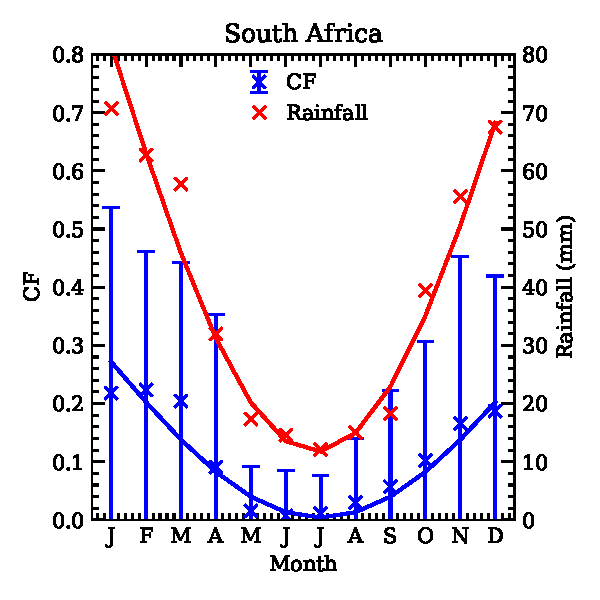
\includegraphics[width=0.85\linewidth]{figures/cf_rainfall_capetown}
    \caption{South Africa}
    \label{fig:cf_rf_south}
  \end{subfigure}
  \begin{subfigure}{\linewidth}
    \centering
    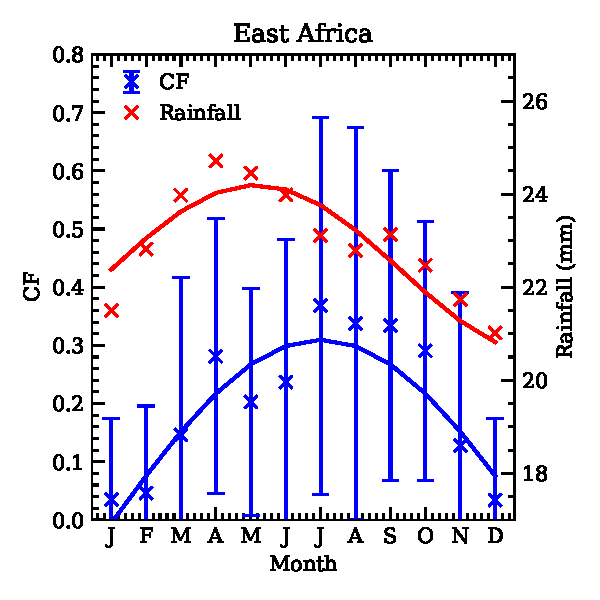
\includegraphics[width=0.85\linewidth]{figures/cf_rainfall_eastafrica}
    \caption{East Africa}
    \label{fig:cf_rf_east}
  \end{subfigure}
  \caption{Monthly averages of cloud fraction over the period
    $2008-2017$ (blue), with associated uncertainties and a fitted
    sinusoidal curve with fixed period $T=12$ months. Also shown are
    monthly averages of rainfall data over the period $1991-2015$
    (red) for South Africa (top) and Ethiopia (bottom) and fits of
    sinusoidal curves with period again fixed at $T=12$ months.}
  \label{fig:cf_rf}
\end{figure}

\subsubsection{SSTA}
Figure \ref{fig:cf_temporal} shows the dynamics of cloud coverage
anomalies between March 2008 and July 2017 for South Africa (Figure
\ref{fig:cf_t_south}) and East Africa (Figure \ref{fig:cf_t_east}) and
associated uncertainty, indicated by the shaded region. Also plotted
are the ONI and the relevant Indian Ocean SST anomalies (SSTAs) -- SWIO
for South Africa and WTIO for East Africa.
\begin{figure*}
  \centering
  \begin{subfigure}{\textwidth}
    \centering
    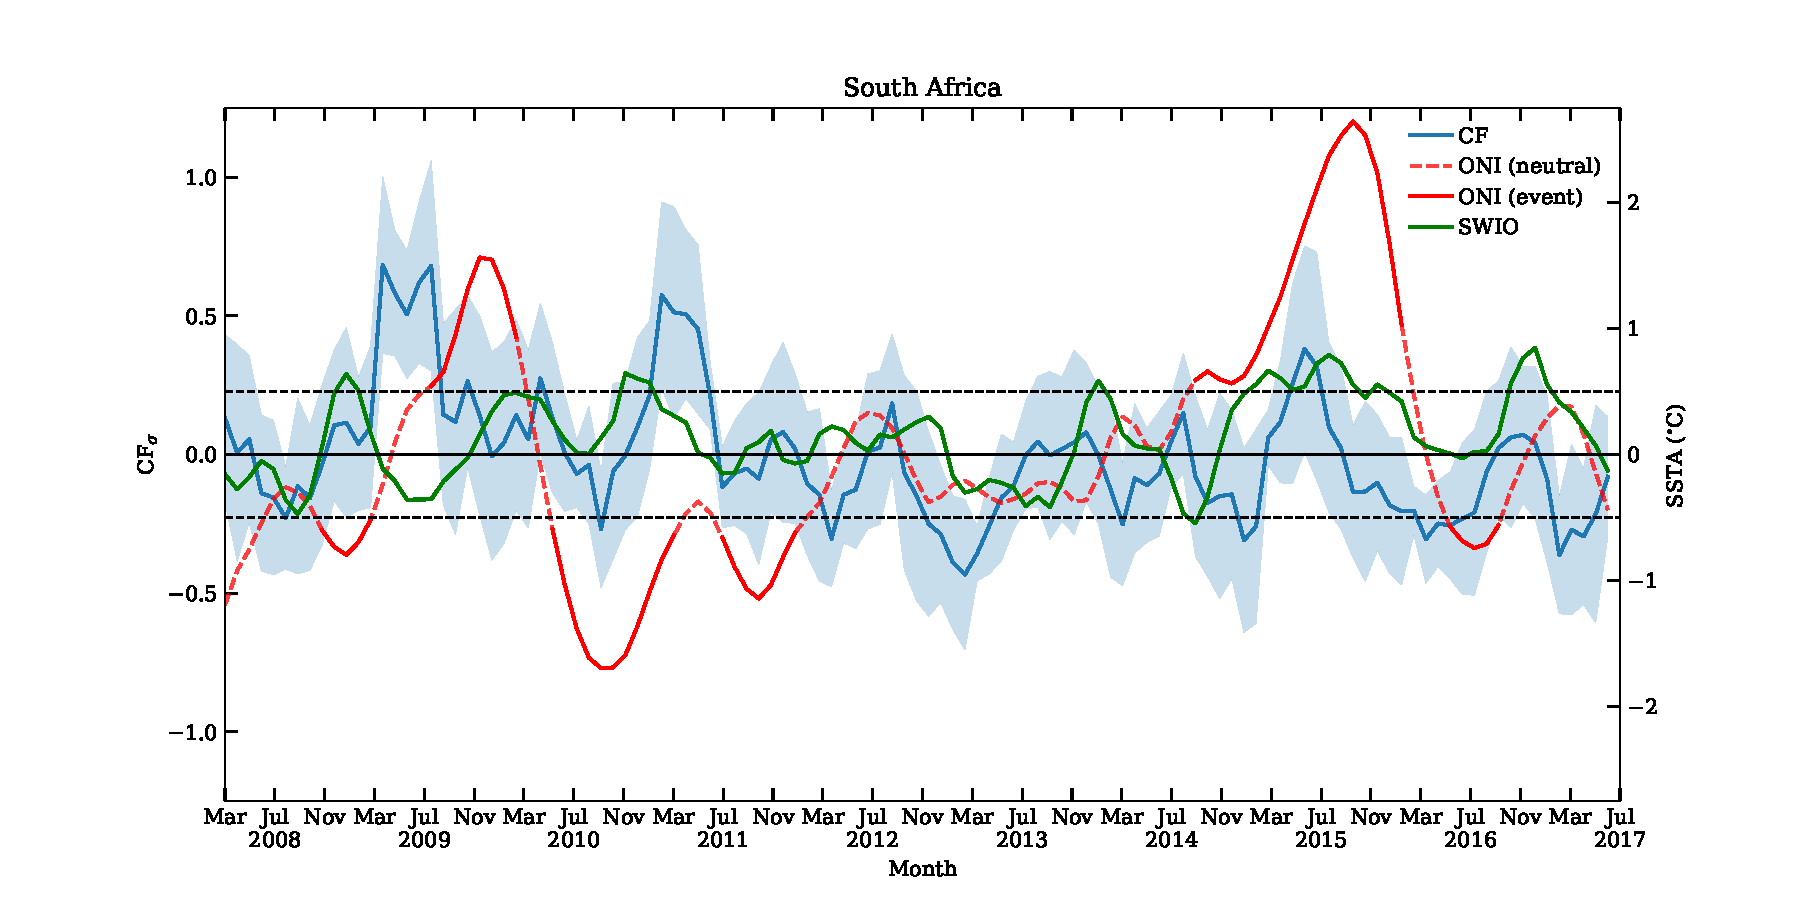
\includegraphics[width=0.85\textwidth]{figures/cf_oni_io_capetown_5window_median}
    \caption{South Africa}
    \label{fig:cf_t_south}
  \end{subfigure}
  \begin{subfigure}{\textwidth}
    \centering
    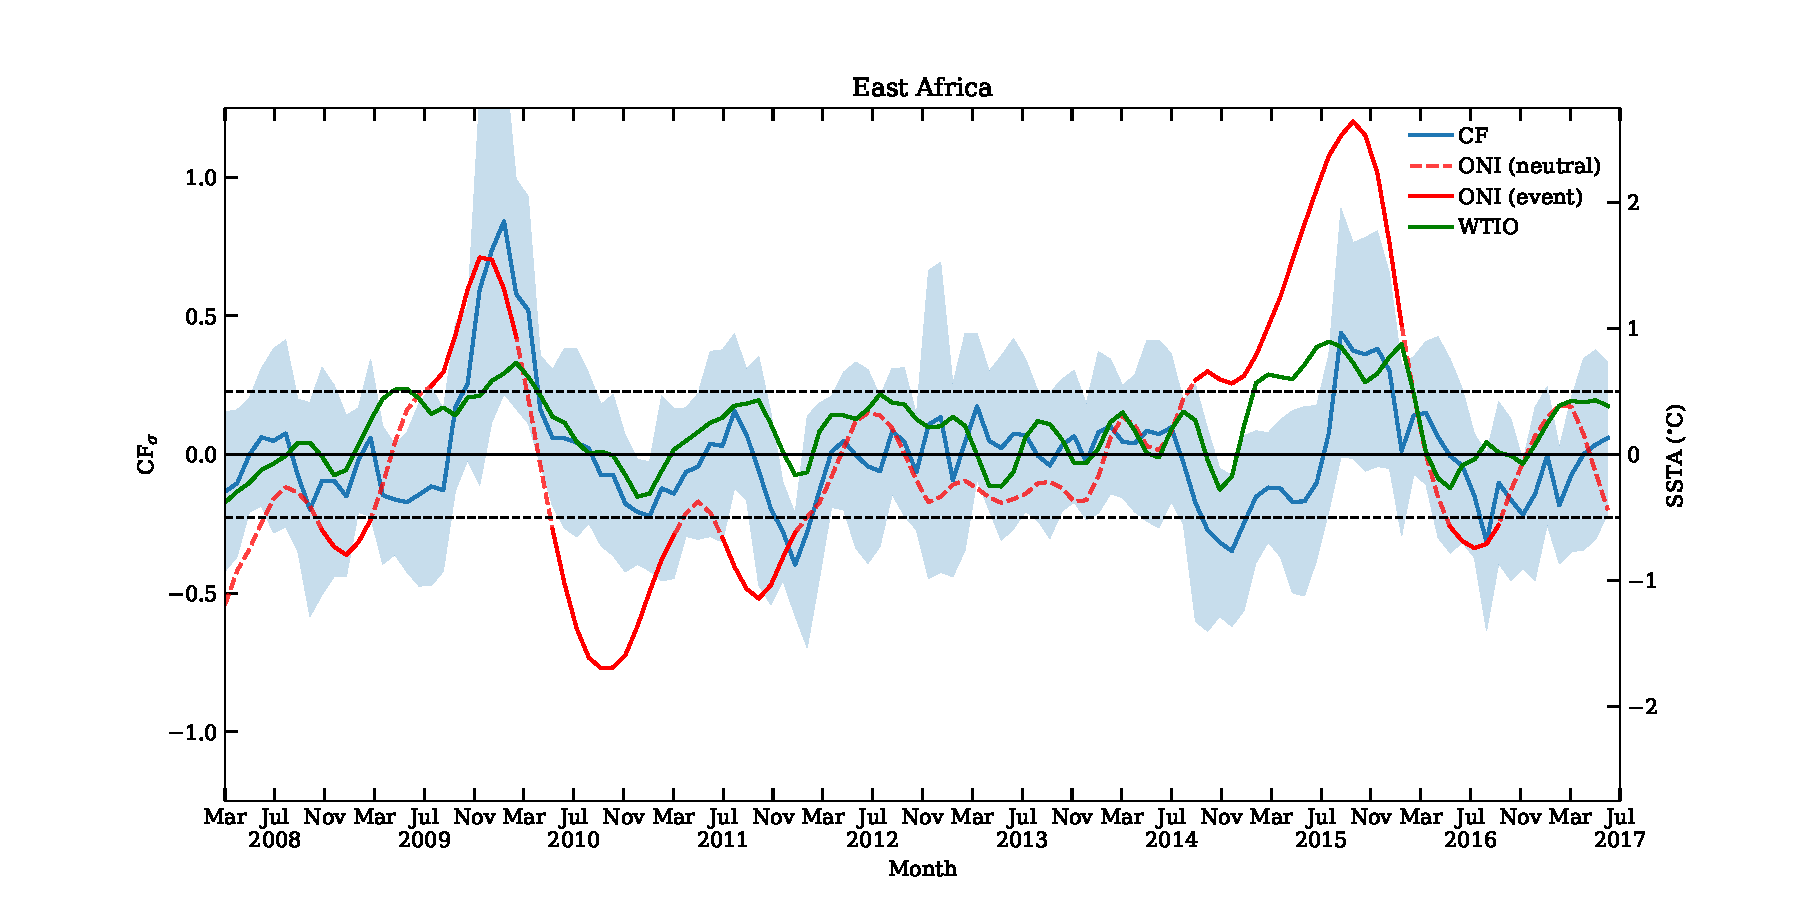
\includegraphics[width=0.85\textwidth]{figures/cf_oni_io_eastafrica_5window_median}
    \caption{East Africa}
    \label{fig:cf_t_east}
    \end{subfigure}
  \caption{Time series of cloud fraction anomalies (blue) and
    uncertainty (shaded blue) from March 2008 to July 2017. Overlaid
    are the ONI (solid red line during ENSO events, dashed red line
    otherwise) and Indian Ocean SST anomalies (SSTA) for the relevant
    part of the Indian Ocean (green, SWIO for South Africa and WTIO
    for East Africa). Dashed black lines indicate the $\pm0.5^{\circ}$C
    threshold for declaring ENSO events. Top panel: South
    Africa. Bottom panel: East Africa. We can see that for South
    Africa, the cloud fraction anomalies are generally anti-correlated
    with ONI during ENSO events with a lag of $\sim2$ months, aside from
    July 2015, where the effect on cloud fraction anomalies appears to
    be dominated by the SWIO SSTAs. For East Africa, cloud fraction
    anomalies appear to be strongly correlated with both ENSO events
    and WTIO SSTAs.}
  \label{fig:cf_temporal}
\end{figure*}

From Figure \ref{fig:cf_t_south} we can see that in many instances, the
cloud fraction anomalies for South Africa appear to be out of phase
with ENSO events, following a lag of $\sim2$ months. For example,
following the peak of the 2010 \nina{} event around November, we
observe a turnaround of cloud fraction anomalies from $-0.25$ to a
peak of $0.5$ by March 2011, which persists until around July of that
year. During the very strong \elnino{} event beginning in November
2014 we observe a positive cloud fraction anomaly, coinciding with
extended periods of positive SWIO SSTAs.

Looking at Figure \ref{fig:cf_t_east} we observe strong positive cloud
fraction anomalies following the peak of the \elnino{} events of
2009/2010 and 2014/2015, again with a lag of $\sim2$ months. However,
cloud fraction anomalies are suppressed during the growth of the
2014/2015 \elnino{} and appear to instead follow the negative WTIO
SSTAs. Negative cloud fraction anomalies are observed during the
2008/2009, 2010/2011, 2011/2012 and 2016 \nina{} events, exhibiting
the same time lag. During all of these periods, apart from the 2016
\nina{}, negative WTIO SSTAs are also present.

\subsection{Vegetation}
To maximise the benefits of using remote sensing, we have divided our
analysis of vegetation coverage into two parts: spatial response and
temporal dynamics.

\subsubsection{Spatial}
Figures \ref{fig:ndvi_sp_south} and \ref{fig:ndvi_sp_east} show the
spatial response of NDVI for South and East Africa respectively. The
images are divided up into two seasons, December-January-February
(DJF) and June-July-August (JJA) as these correspond to the extrema of
the seasonal modulation of cloud coverage (Figure \ref{fig:cf_rf}) and
so are the times when any anomalies will likely be most visible. Each
column is then further divided up into whether \elnino{}, \nina{} or
neutral conditions are present.

\begin{figure*}
  \centering
  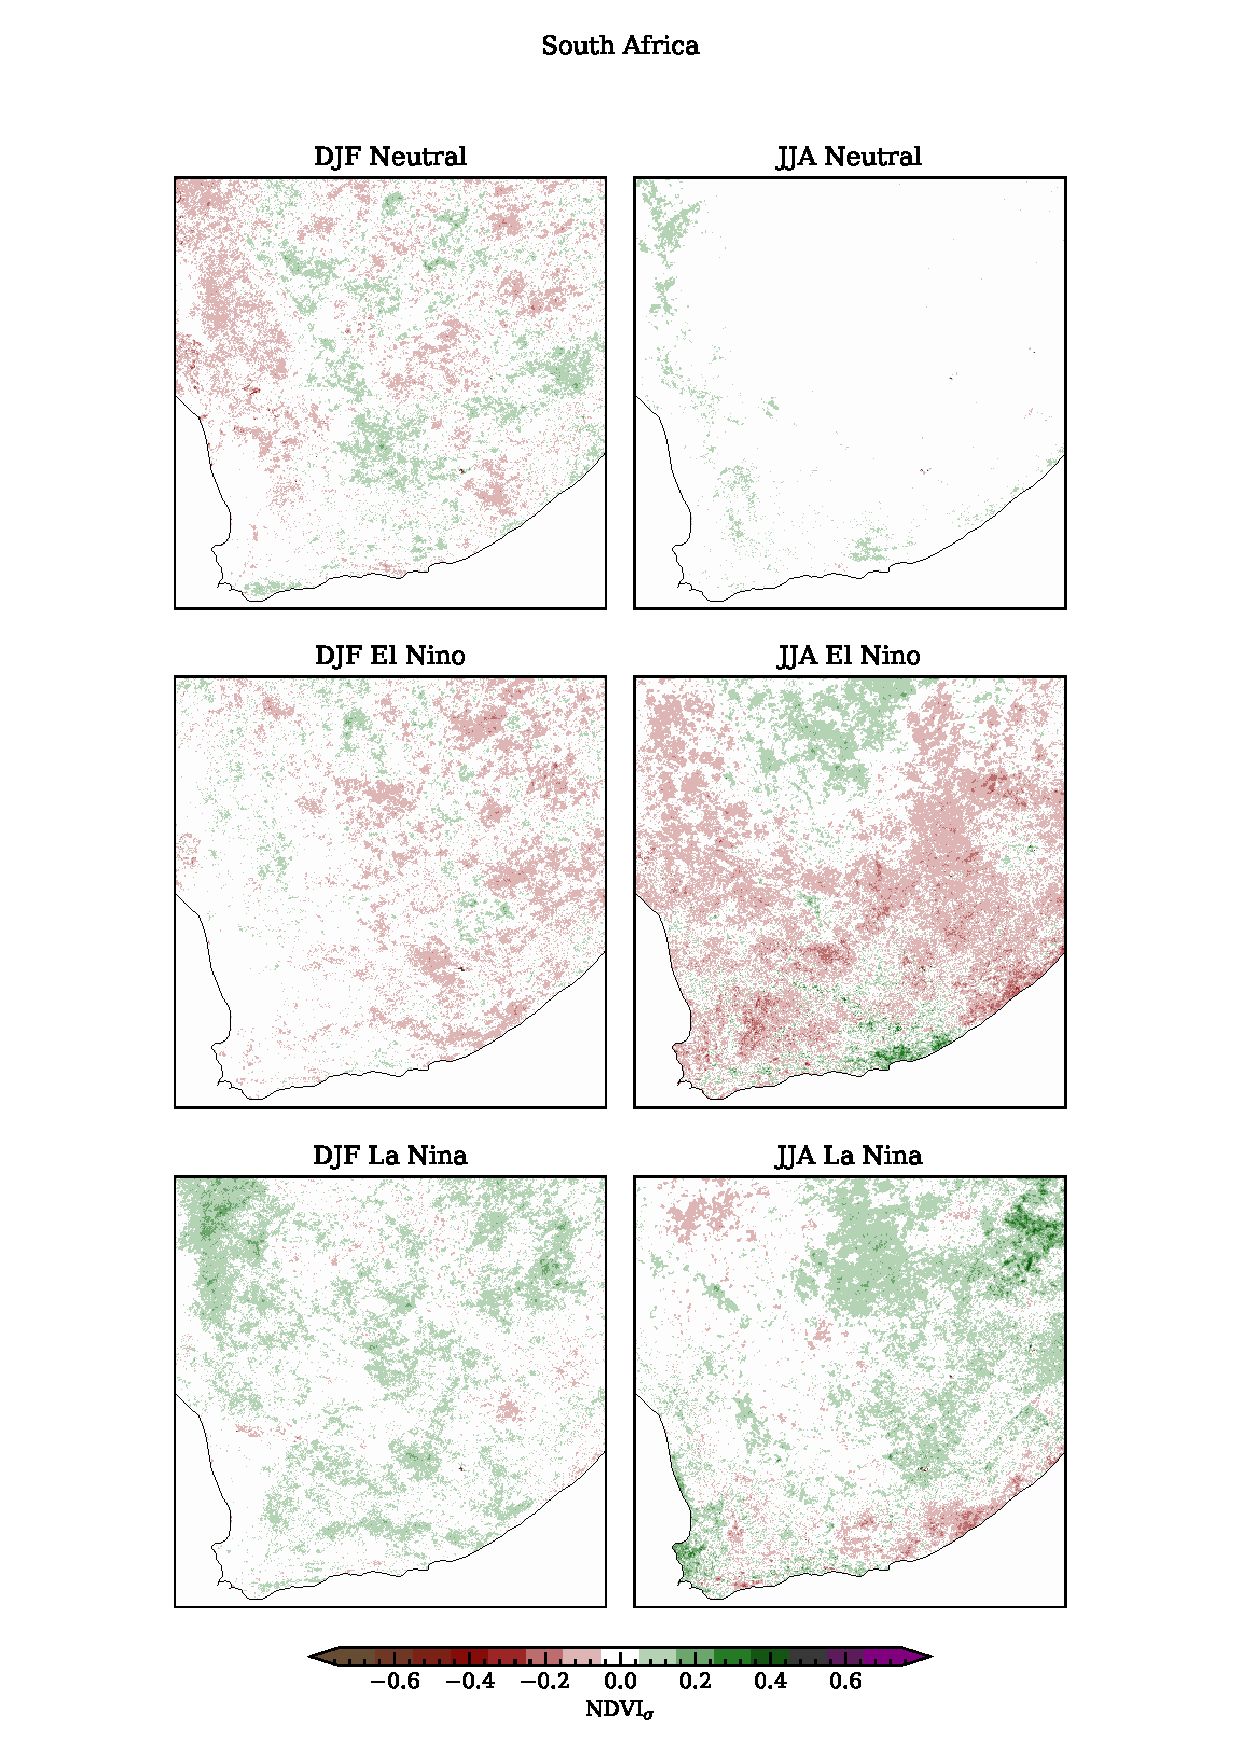
\includegraphics[height=0.9\textheight]{figures/ndvi_spatial_seasonal_anomalies_capetown}
  \caption{Spatial distribution of NDVI anomalies for South
    Africa. Three monthly means are taken for
    December-January-February (DJF) and June-July-August (JJA) and
    averaged again according to which phase of ENSO was present at the
    time.}
  \label{fig:ndvi_sp_south}
\end{figure*}

\begin{figure*}
  \centering
  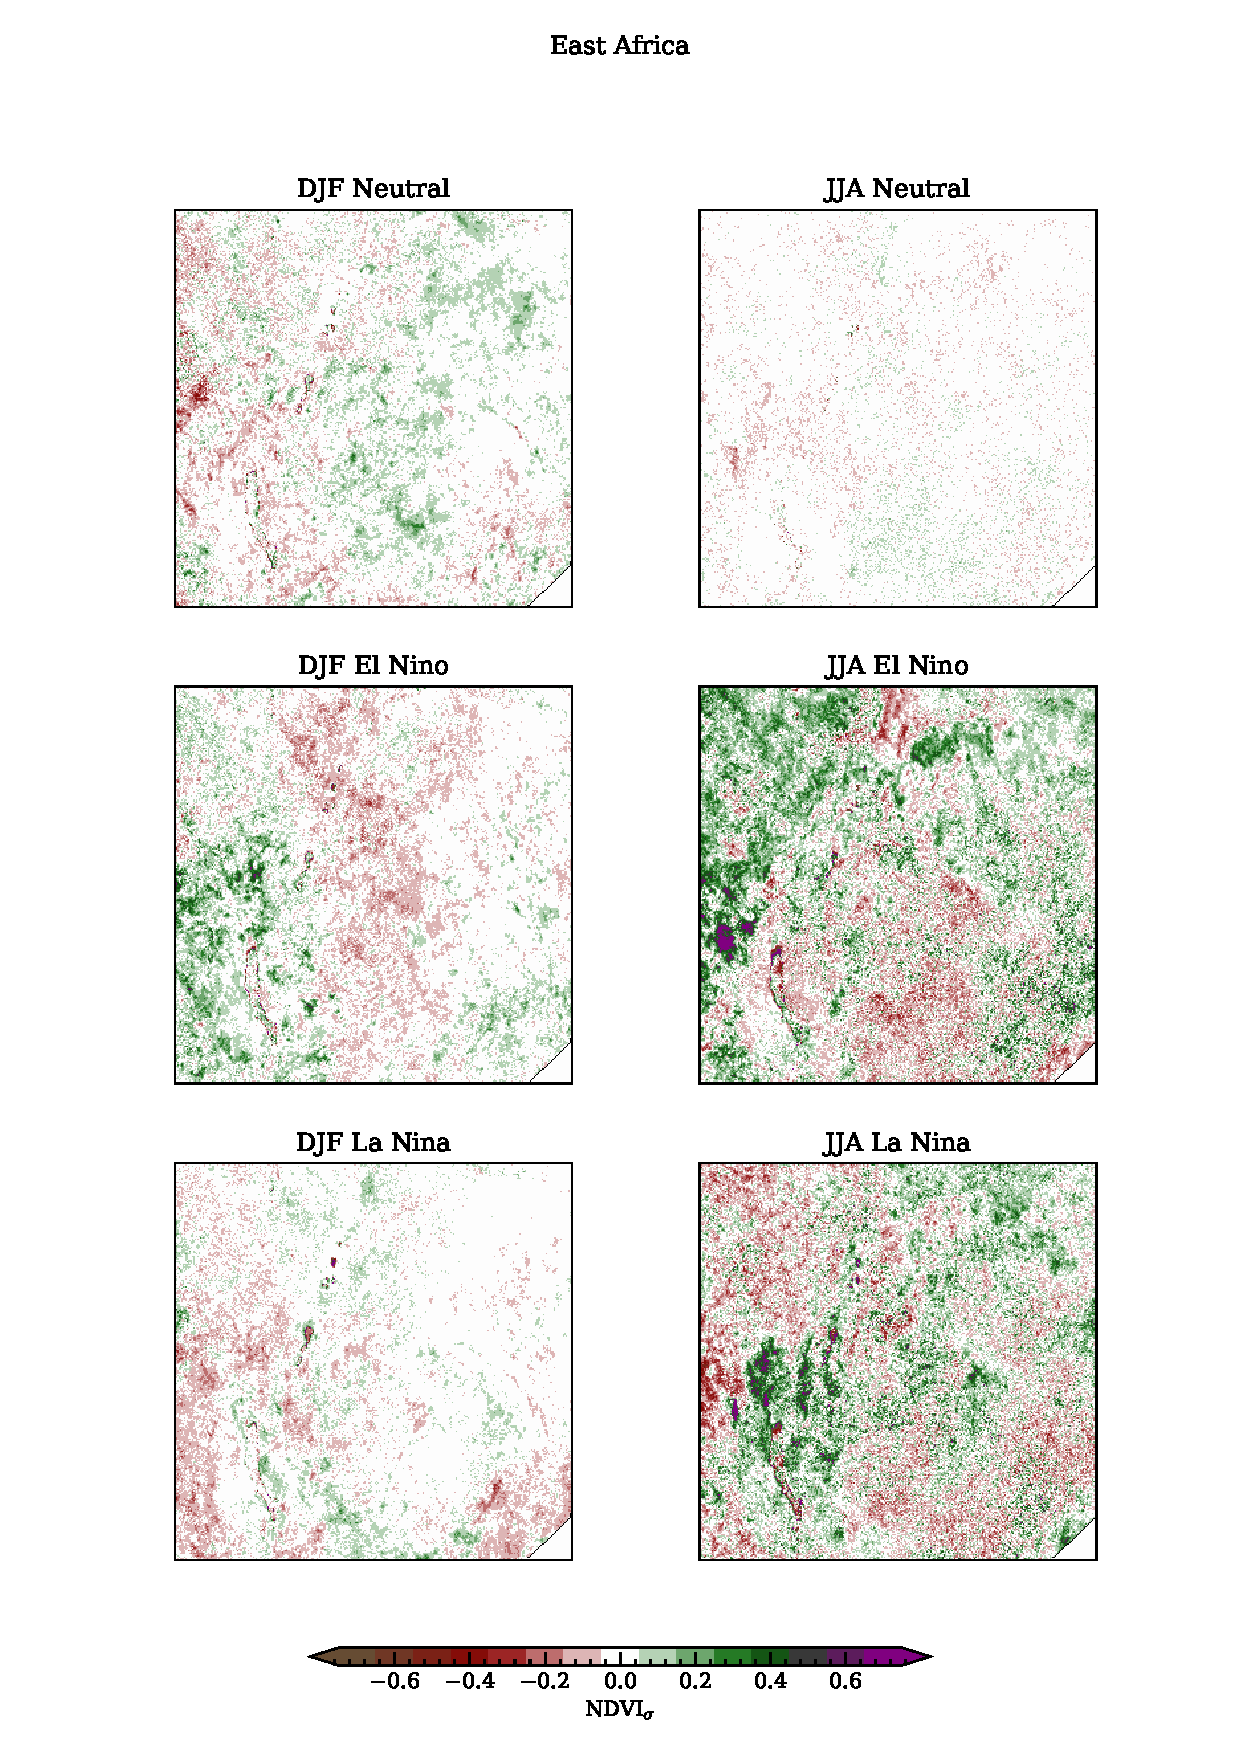
\includegraphics[height=0.9\textheight]{figures/ndvi_spatial_seasonal_anomalies_eastafrica}
  \caption{Spatial distribution of NDVI anomalies for East
    Africa. Three monthly means are taken for
    December-January-February (DJF) and June-July-August (JJA) and
    averaged again according to which phase of ENSO was present at the
    time.}
  \label{fig:ndvi_sp_east}
\end{figure*}

Looking first at South Africa, the top panels of Figure
\ref{fig:ndvi_sp_south} show that during neutral periods relatively
small, evenly distributed anomalies are present during DJF, while for
JJA there are are mostly no anomalies, aside from some small positive
anomalies in the west. In the middle panels we can see that during
\elnino{} periods we observe a dearth of vegetation. These negative
anomalies are confined mostly to the east in DJF, while in JJA the
anomalies cover most of the region, with some positive anomalies
appearing in the north and along south-eastern coastal
regions. Finally, the bottom panels show that during \nina{} periods
we observe an excess of vegetation, distributed fairly evenly across
the region for both periods. Some negative anomalies appearing in
the north-west and along the south-eastern coast during JJA, in similar places to the positive anomalies seen in JJA \elnino{}.

Moving now to East Africa, the top panels show a similar pattern to
Figure \ref{fig:ndvi_sp_east} namely that in neutral periods anomalies
are small and dispersed during DJF, although there does appear to be a
tendency for negative anomalies to appear in the south and positive
anomalies in the north. In JJA, anomalies are again essentially
absent. For \elnino{} periods, the middle left panel shows that, during
DJF, there are positive anomalies in the east, south-east and
south-west and negative anomalies in the centre, stretching from north
to south. During JJA, the positive anomalies in the east are very
large and spatially concentrated, as are the negative anomalies in the
north; elsewhere positive and negative anomalies are interspersed
adjacently. During \nina{} events, positive anomalies concentrated
mostly in the south dominate during DJF. In JJA there is a mix of
pockets of high positive anomaly (e.g. the west and north-east) and
positive anomaly (e.g. far west, north west).

% Move stuff about ENSO events to results?

% Some of the claims in the concluding paragraph of SSTA may be
% slightly grandiose

\section{Discussion}
\label{sec:disc}
\subsection{Thresholding}
\label{sec:disc:thresh}
In Section \ref{sec:method:thr} we described our method for
thresholding images, namely using Otsu's method. Figure \ref{fig:allp}
is illustrative of the efficacy of this method, applying it to all
land pixels for a single day (1/6/2008). Figure \ref{fig:allp_raw}
shows the raw image from EUMETSAT, where cloud is clearly visible over
western and equatorial Africa. Figure \ref{fig:allp_hist} shows the
distribution of land pixels in Figure \ref{fig:allp_raw}. It is not
clear whether the distribution is bimodal or log-normal, though it
could be said that there are two peaks: one at a pixel value of $\sim50$
and the other at a pixel value of $\sim110$. The broadness of this
distribution is caused by taking values from the entire image, whereas
in fact some places on the planet will be brighter in VIS0.8 than
others. We have then applied an Otsu threshold to categorise pixels as
`land' or `cloud', shown as white and green on the histogram. This is
a crude way of doing things, and is only done to illustrate the
process -- in reality, the Otsu threshold is calculated for \emph{each}
pixel from the distribution of its values over a period of time, so
the threshold value is more accurately scaled to that pixel. Figure
\ref{fig:allp_im} shows the land pixels from Figure \ref{fig:allp_raw}
where each pixels colour has been assigned according to whether it was
categorised as `land', `cloud' or masked out. Using this very simple
threshold manages to catch most of the cloud in western and equatorial
Africa, although it clearly fails miserably over the Sahara. In our
analysis we have overcome the shortcomings of the thresholding in the
desert by avoiding arid regions.
\begin{figure*}
  \centering
  \subcaptionbox{Raw image from
    EUMETSAT.\label{fig:allp_raw}}
                [0.3\textwidth]
                {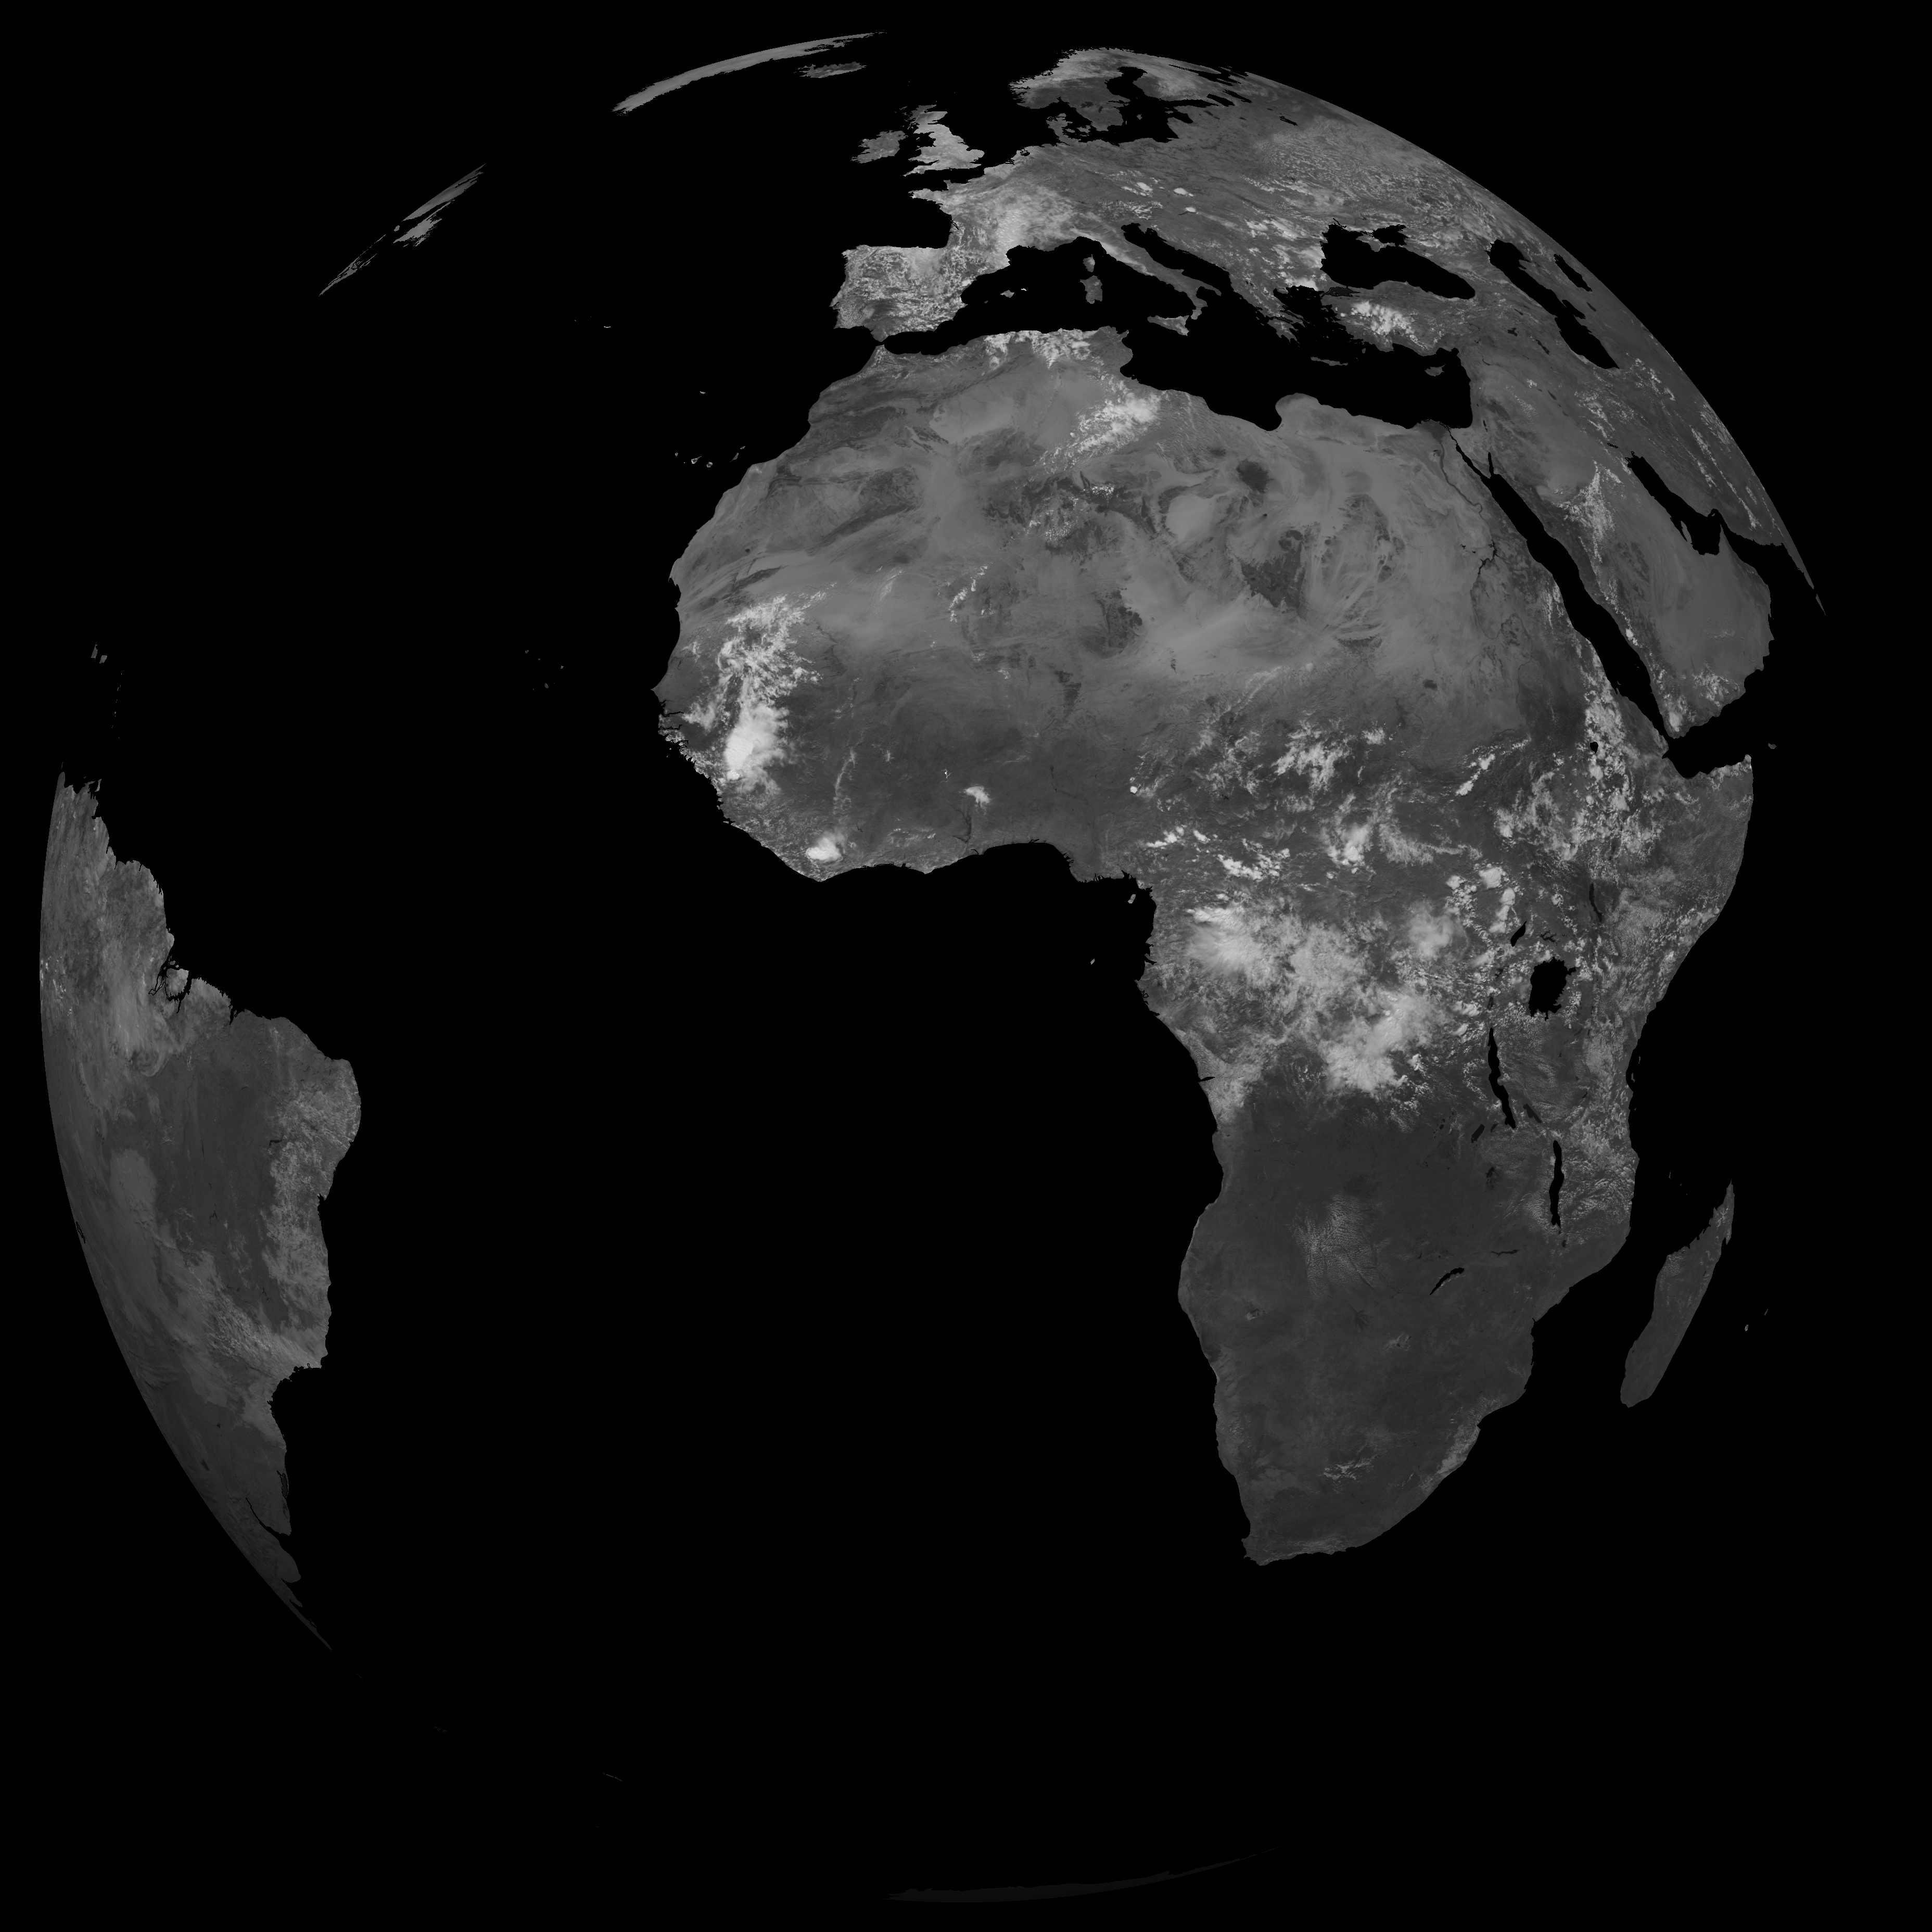
\includegraphics[width=0.3\textwidth]{figures/raw_im_all_pixels_01_06_2008_vis8}}
  ~
  \subcaptionbox{Histogram of the distribution of all the
    land pixels in Figure \ref{fig:allp_raw}. Green
    indicates where a pixel has been classified as `land'
    and white indicates `cloud' and black corresponds to
    masked pixels.\label{fig:allp_hist}}
                [0.33\textwidth]
                {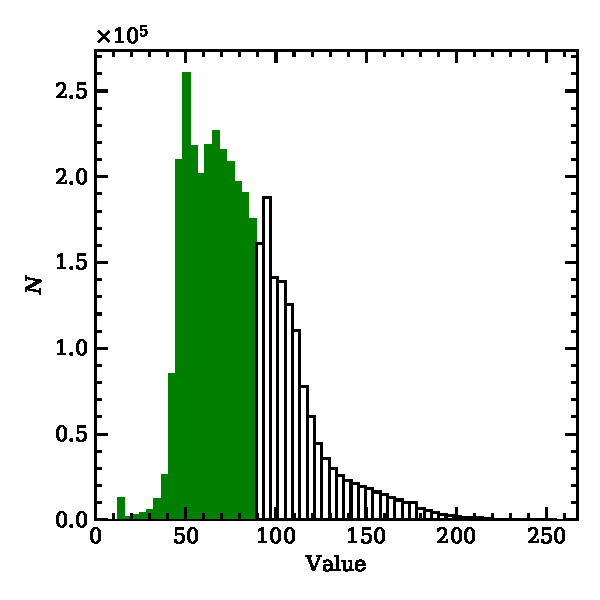
\includegraphics[width=0.33\textwidth]{figures/hist_all_pixels_01_06_2008_vis8}}
  ~
  \subcaptionbox{The image in Figure
    \ref{fig:allp_raw} masked and
    thresholded, so that the colour of each
    pixel corresponds to its classification
    as `land', `cloud' or masked
    out.\label{fig:allp_im}}
                [0.3\textwidth]
                {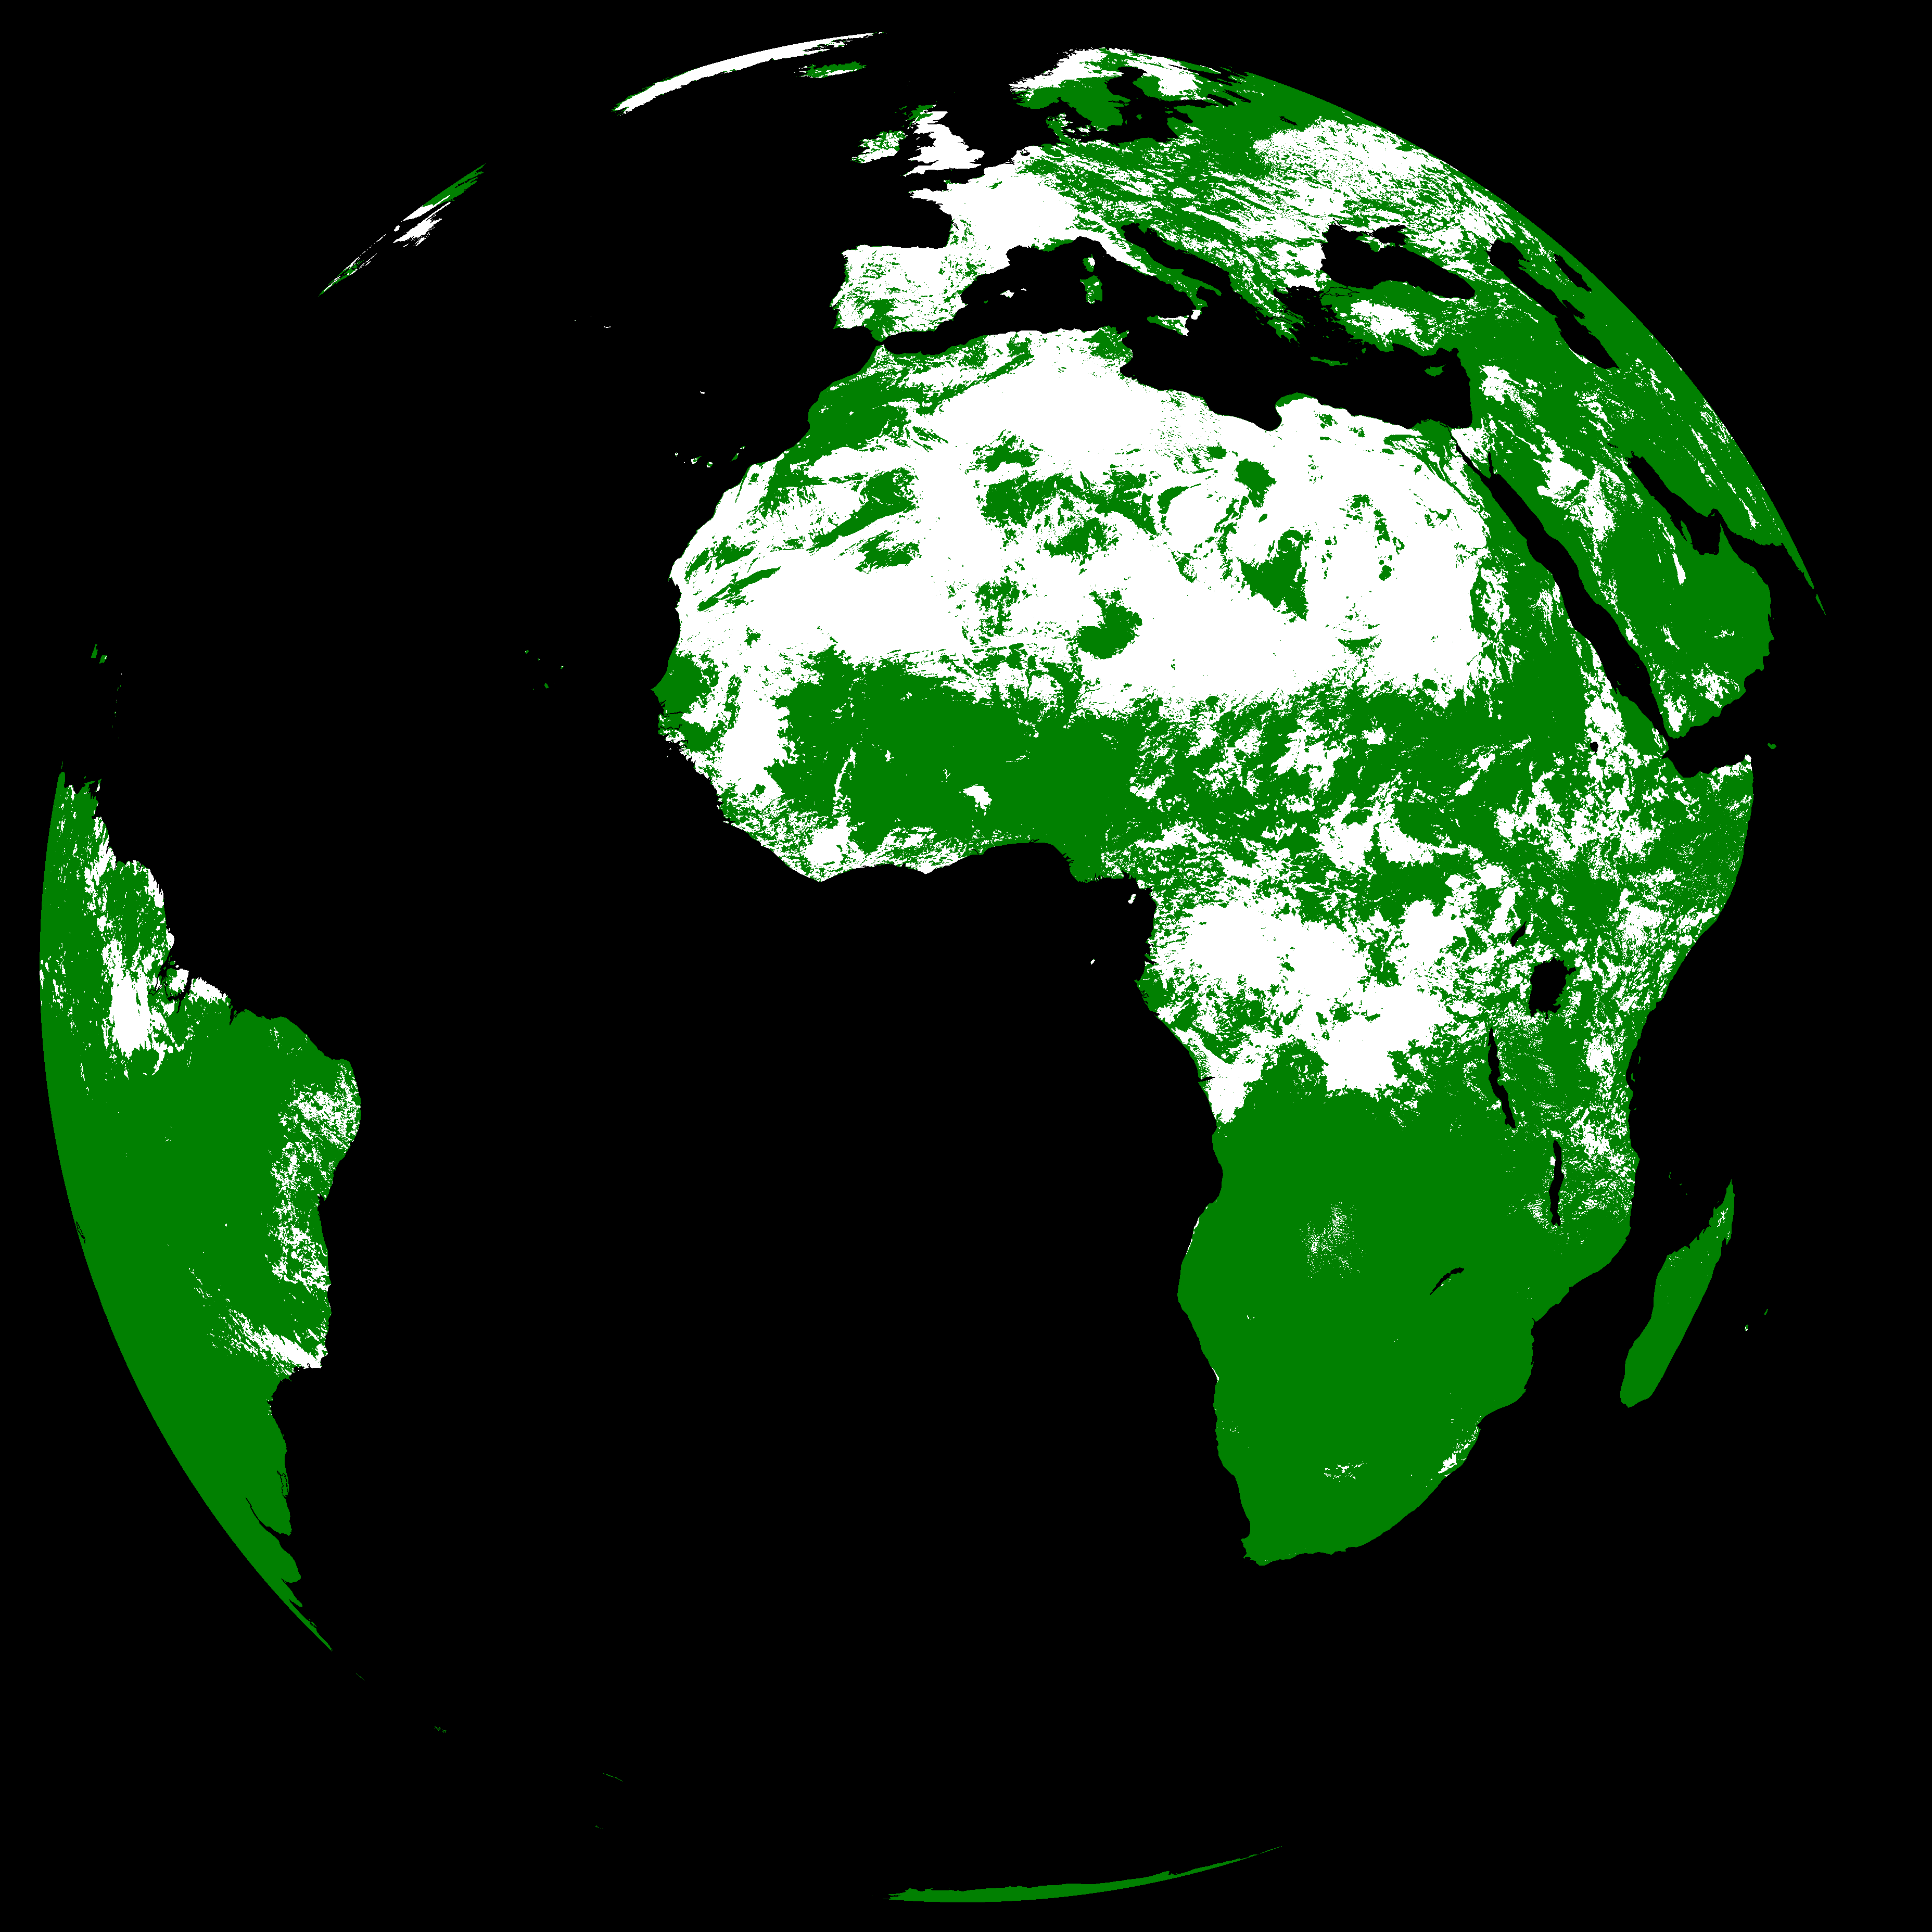
\includegraphics[width=0.3\textwidth]{figures/im_all_pixels_01_06_2008_vis8}}
  \caption{Thresholding of the image for 1/6/2008 in the VIS0.8 band.}
  \label{fig:allp}
\end{figure*}
It is useful to explore thresholding on the entire distribution, but
more relevant to our analysis is to see how it works for single
pixels. Figures \ref{pix_d_south} and \ref{pix_d_east} show the
normalised pixel distributions for South Africa and East Africa, for
three different pixels in the VIS0.6 and VIS0.8 bands. Also shown on
the plot are various statistics of the data, including the value of
the threshold calculated with Otsu's method, the mean of the entire
dataset, the median of the entire dataset, the mean of the data less
than the Otsu threshold and a Gaussian fit of the data less than the
Otsu threshold. It can be seen from the figures, that the fitted
Gaussian agrees fairly well with the data below the Otsu
threshold. This indicates that our method for producing cloud masks is
applicable -- we say that a pixel is classified as clear if it has a
value less than the value of the `ground' pixel plus some
uncertainty. The normal distribution of the values around the `ground'
value is as we expect, because some days the pixel will be in shade
and some days there will be some wispy cloud that we are unable to
detect. Here, the value of the `ground' pixel is the mean and the
uncertainty is the standard deviation of data below the threshold. It
is also interesting to note that the median returns a similar value to
the mean of the data below the threshold, although it does tend to
slightly overestimate.
\begin{figure*}
  \centering
  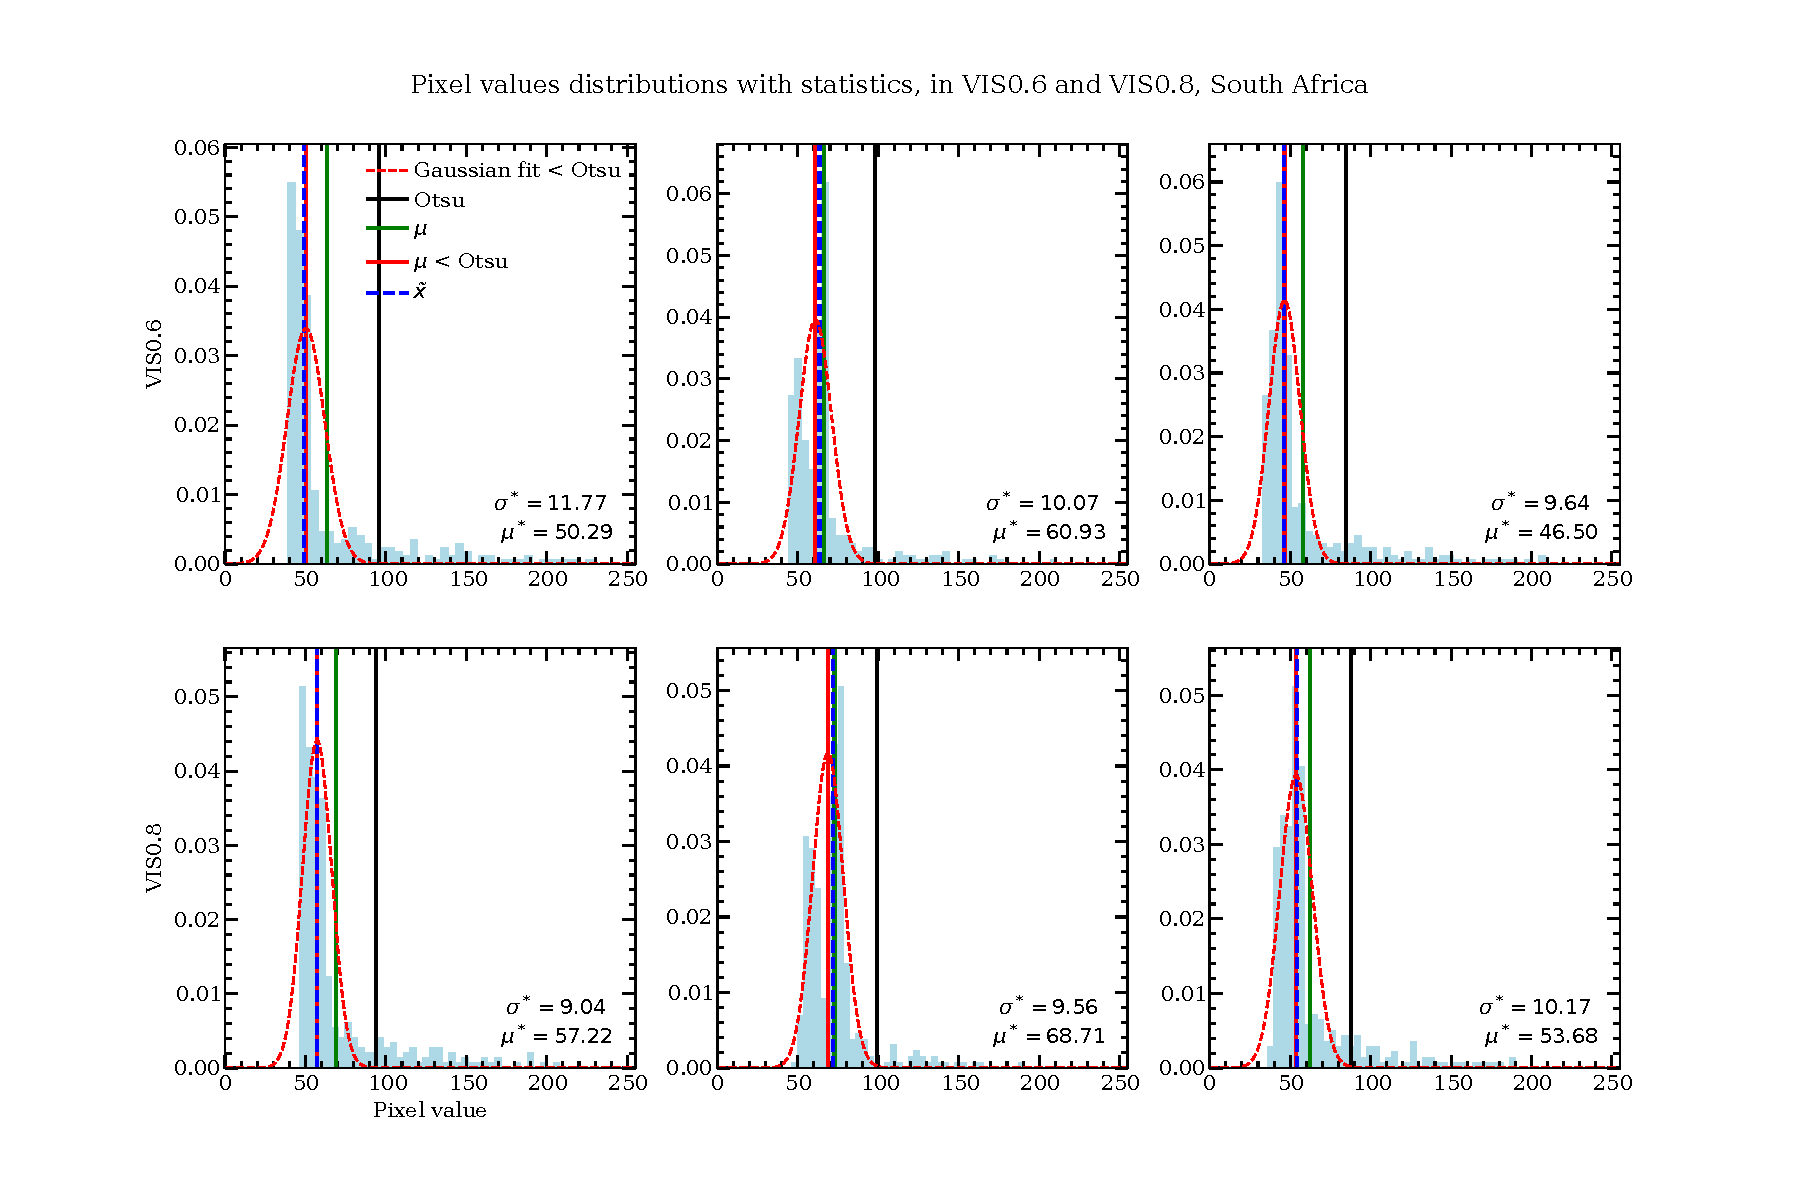
\includegraphics[width=\textwidth]{figures/pixel_distributions_stats_capetown}
  \caption{Normalised pixel distributions South Africa in the VIS0.8
    and VIS0.6 bands, for three pixels. Shown are the Otsu threshold
    (black), the mean of the entire dataset (green), the median of the
    entire dataset (dashed blue), the mean of the values below the
    Otsu threshold (red) and a Gaussian fit to the data below the Otsu
    threshold (dashed red). In the bottom right are the values for the
    mean $\mu$ and standard deviation $\sigma$ of the fitted Gaussian. The
    key point to note is how well the Gaussian fits the data below the
    threshold. This indicates that our method of using the mean of the
    values below the Otsu threshold to calculate a cloud free image
    (with the standard deviation as the uncertainty) is sound. Also
    interesting to note is how close the median is to this mean value,
    although it is usually an overestimate.}
  \label{fig:pix_d_south}
\end{figure*}

\begin{figure*}
  \centering
  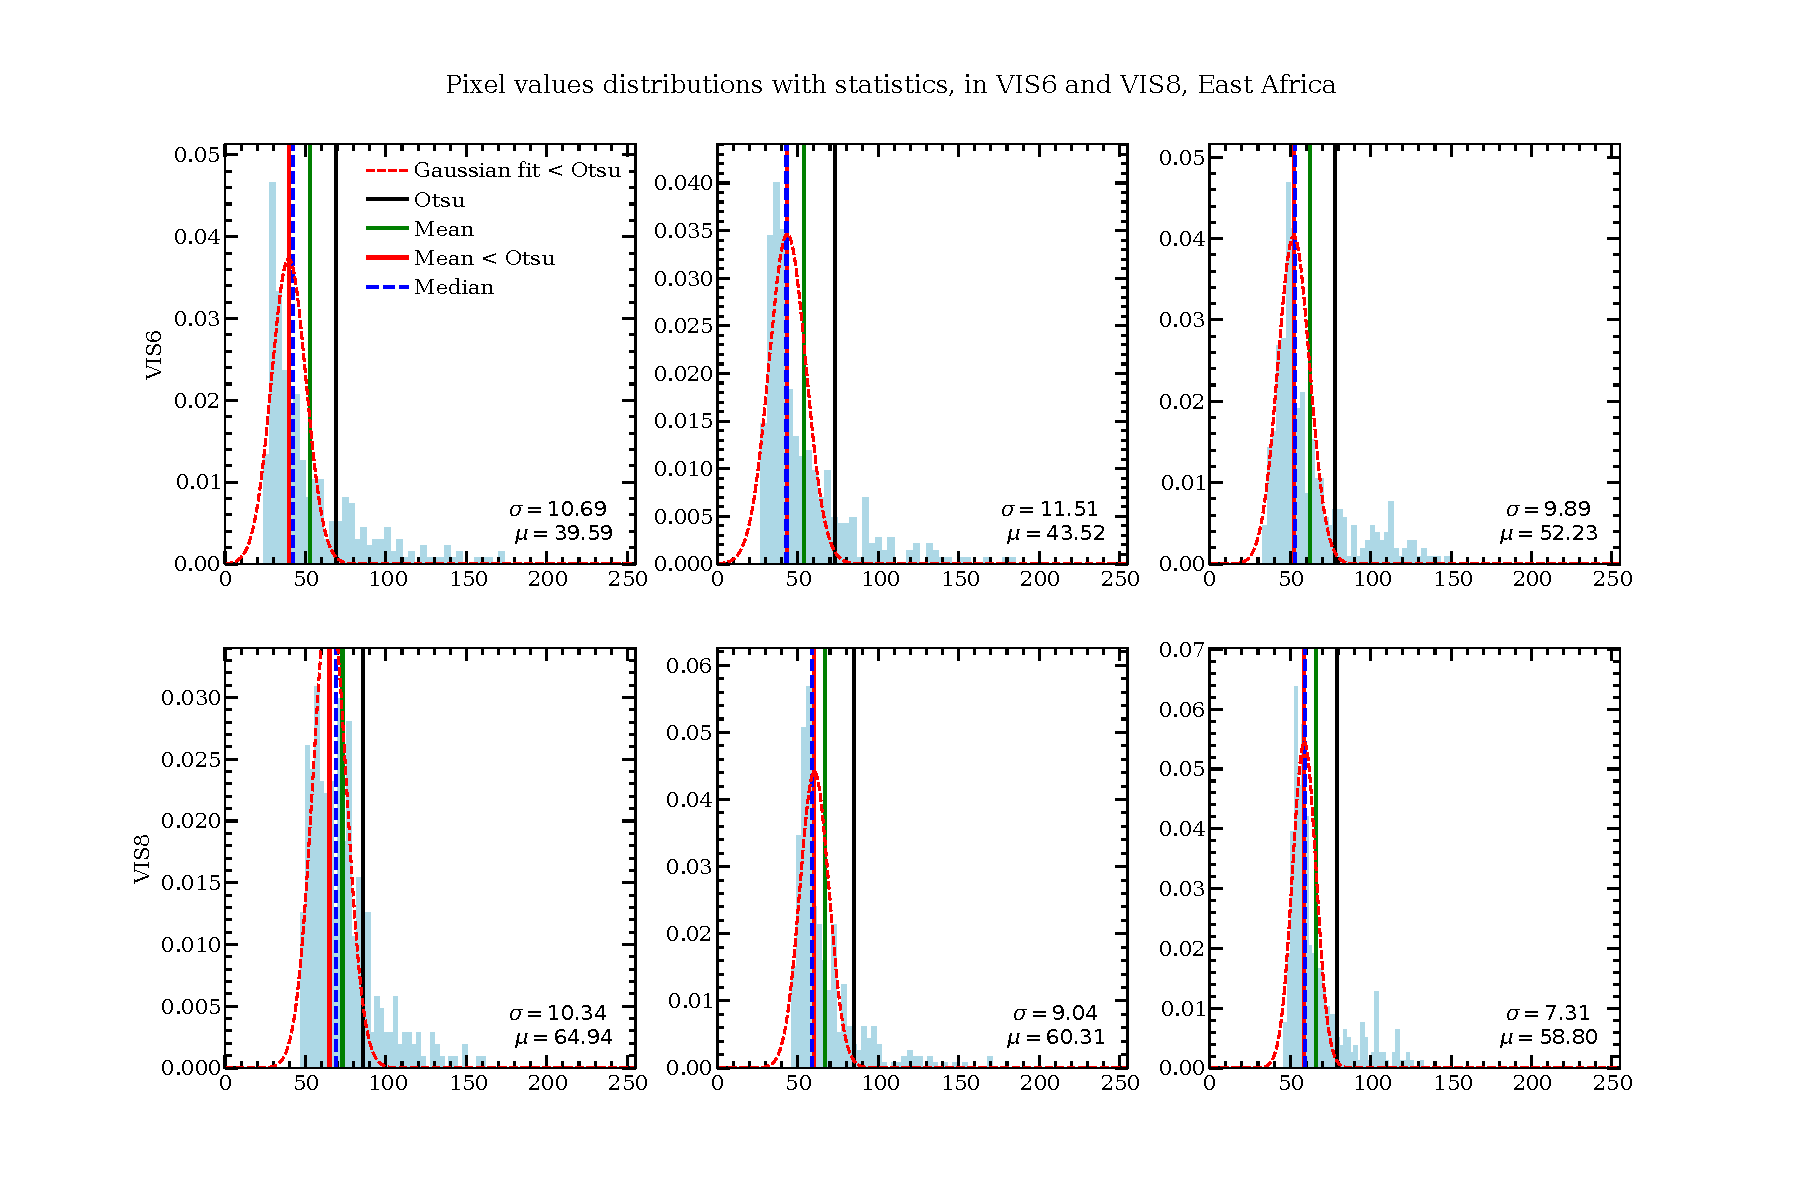
\includegraphics[width=\textwidth]{figures/pixel_distributions_stats_eastafrica}
  \caption{As in Figure \ref{fig:pix_d_south}, but for East Africa.}
  \label{fig:pix_d_east}
\end{figure*}

\subsection{Cloud coverage}
\label{sec:disc:cc}
When calculating monthly values for cloud fraction, we have to average
over all of the days for a given month. In calculating this average we
could use either the mean or the median, and then estimate the
uncertainty based on the standard deviation or interquartile range
(IQR). Figure \ref{fig:cf_dist_south} shows the distribution of cloud
fraction values within a month for South Africa, and Figure
\ref{fig:cf_dist_east} shows the same but for East Africa. The
interesting point here is that the distribution changes from being
skewed to looking almost normally distributed, due to the seasonal
modulation (discussed in depth in Section \ref{sec:disc:rain}). Figure
\ref{fig:cf_dist} shows that using the mean as the average and the
standard deviation as an estimate of uncertainty for July (January) in
South Africa (East Africa) is clearly not appropriate, as they are
skewed by the long tail. For these months the median and IQR do a much
better job of selecting the average and its uncertainty. In January
(July) for South Africa (East Africa) the mean and standard deviation
could be used, but the median is still useful even when the data
appear to be normally distributed and it is much better to use a
statistical measure that is appropriate for all the data, rather than
one that is suited to one part of the dataset but completely off for
the rest.
\begin{figure*}
  \centering
  \begin{subfigure}{0.45\textwidth}
    \centering
    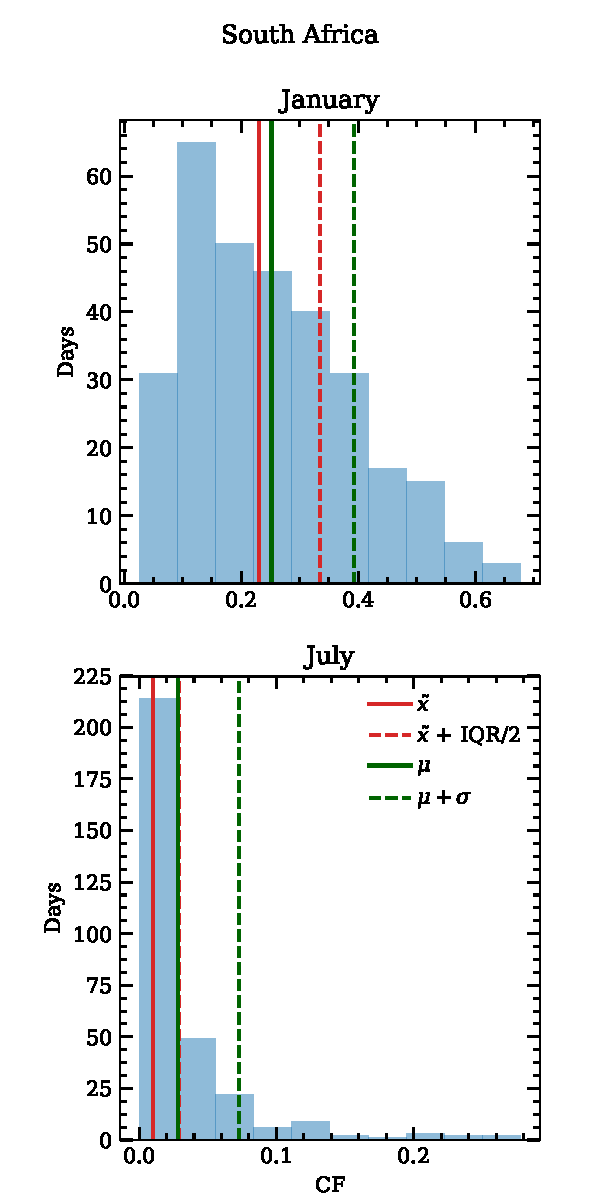
\includegraphics[width=\textwidth]{figures/cf_monthly_dist_capetown}
    \caption{South Africa. Note how in January the cloud fractions
      appear to be normally distributed, while in July they are skewed
      toward lower values. This is due to seasonal modulation, which
      is discussed in depth in Section \ref{sec:disc:rain}.}
    \label{fig:cf_dist_south}
  \end{subfigure}
  ~
  \begin{subfigure}{0.45\textwidth}
    \centering
    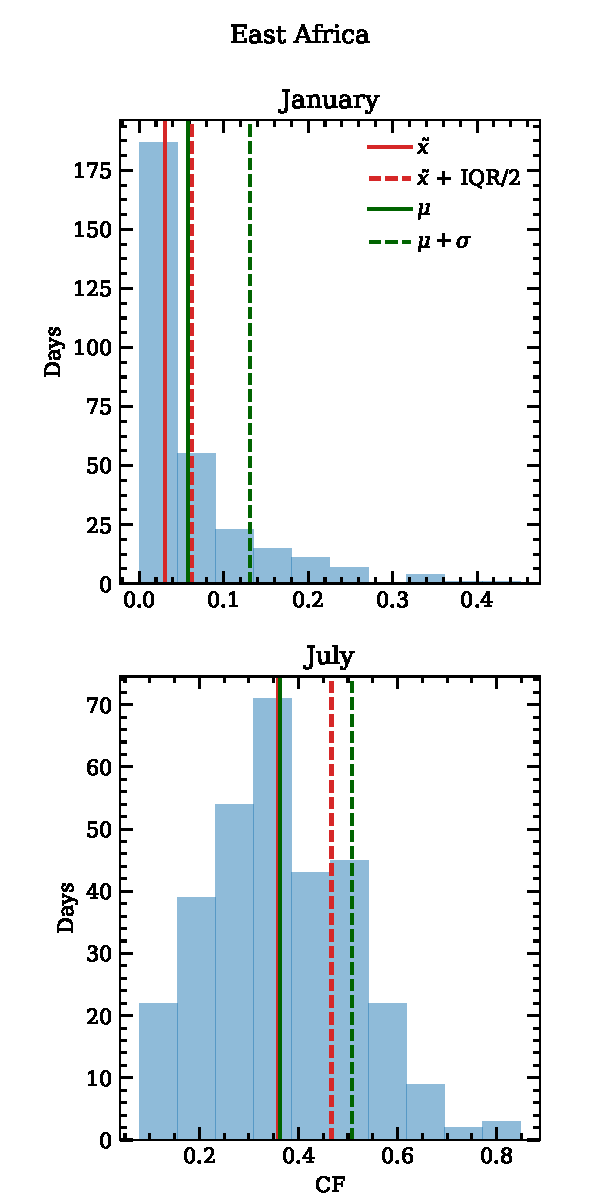
\includegraphics[width=\textwidth]{figures/cf_monthly_dist_eastafrica}
    \caption{East Africa. Note how the distributions are swapped
      compared to Figure \ref{fig:cf_dist_south}. Here the values for
      January are skewed toward lower values, while the values for
      July look more normally distributed.}
    \label{fig:cf_dist_east}
  \end{subfigure}
  \caption{Distribution of cloud fraction values for South Africa and
    East Africa. Top: distribution of all values for January, over the
    years 2008--2017. Bottom: distribution of all values for July, for
    the same year range. Shown in solid red is the median values
    $\tilde{x}$, dashed red the median and half the interquartile
    range (IQR), solid green the mean $\mu$ and dashed green the mean
    and one standard deviation $\sigma$.}
  \label{fig:cf_dist}
\end{figure*}

\subsubsection{Rainfall}
\label{sec:disc:rain}
Here we discuss the relationship between cloud coverage and rainfall,
as shown in Figure \ref{fig:cf_rf}. For South Africa (Figure
\ref{fig:cf_rf_south}) it is clear that cloud coverage follows the
same seasonal modulation as rainfall. The rainy season
(November--March) coincides with winter in the southern hemisphere and
the dry season (April--October) with summer. For East Africa the dry
season (December--January) falls in the northern hemisphere winter,
while the rainy season (March--July) falls mostly in summer. The
overall trend of cloud coverage and rainfall is similar here, but
there is some slight disagreement as to where the peak lies. This
neatly highlights one of the benefits of using cloud coverage
determined via remote sensing as a proxy over rainfall data, for
studying general trends. Precipitation data is inherently
inhomogeneous -- there must be a station located somewhere to detect
the rain. For Figure \ref{fig:cf_rf_east} the rainfall station was
located in Ethiopia, while the cloud coverage data is calculated by
taking a box average over the whole of Ethiopia, and parts of Kenya
and Somalia too. Hence we can get a much better idea of the
\emph{general} rainfall dynamics, compared to the \emph{local}
information garnered from precipitation data \footnote{This does not,
  of course, mean that having local data is not useful in different
  situations, for example in comparing rainfall between different
  types of land.}. East Africa is a complex climatic system but, as
the rainfall variability is spatially coherent and driven by
global-scale dynamics, it is reasonable to study the region on the
large scale \citep{nicholson1996b}.
  
%% A key point to note is that any climate effects will depend on what would usually be happening in that season.

%% An interesting point to note is that South African rainfall varies by over 50mm while East African rainfall varies by around 5mm. Drought?

\subsubsection{SSTA}
\label{sec:disc:ssta}
Here we will discuss how cloud coverage responds to SSTAs, beginning
with South Africa (Figure \ref{fig:cf_t_south}). Between July 2009 --
March 2010 and November 2014 -- May 2016 the ENSO is in its warm phase,
\elnino{}. If there is a response to the positive ONI in 2009/2010,
then Figure \ref{fig:cf_t_south} indicates that it is insignificant in
our data. During the 2014--2016 \elnino{} period we observe negative
cloud fraction anomalies from November 2014 which switch to positive
cloud fraction anomalies around January 2015. In July 2015, the cloud
fraction anomalies peak and turn around again, steadily decreasing
toward a minimum in March 2016, roughly 3 months after the ONI peaked
in December 2015. Important to note is that in the same time period
that the positive cloud fraction anomalies peak, strong positive SWIO
SSTAs $>0.5\degc$ are also present. Perhaps here the dearth of cloud
coverage that we expect to see in South Africa due to an \elnino{}
event is countered by enhanced SSTAs in the SWIO before the strong ONI
again triumphs in suppressing cloud coverage.

In our time range there are technically four \nina{} periods: November
2008 -- March 2009, June 2010 -- May 2011, July 2011 -- March 2012 and
August 2016 -- December 2016. Two of the periods are separated by only
a month where the ONI dipped to $-0.4\degc$. Following the peak of the
2008/2009 \nina{} in January 2009, there was a significant spike in
the cloud fraction in March 2009.  This positive anomaly is present
despite negative SWIO SSTAs. Similarly, following the peak of the
2010/2011 \nina{} in October 2011, there is a significant positive
cloud fraction anomaly in December of the same year. The 2011/2012 and
2016 \nina{} events both precede positive cloud fraction anomalies by
two months or so, however, due to the large uncertainty on the values,
it would be misguided to label these as significant. It is also worth
noting that the ONI magnitude for the 2011/2012 and 2016 \nina s are
relatively small in comparison to the other events in our time period.

We move now to East Africa, shown in Figure
\ref{fig:cf_rf_east}. Immediately before and during the growth of the
2009/2010 \elnino{} we observe negative cloud fractions. Around
October 2009 the cloud fraction anomalies climb rapidly before peaking
in January 2010 at the largest value we observe in our entire dataset
(CF$_{\sigma}=0.88\pm0.59$). This peak in cloud anomalies comes a month
after the peak of the \elnino{} event in December 2009 and coincides
with positive WTIO SSTAs ($>0.25\degc$), present since March 2009
which become large ($>0.5\degc$) in January 2010. Comparing this
response with that of the 2014--2016 \elnino{}, we find that the
negative anomalies present during the growth of \elnino{} are much
more pronounced. The negative cloud anomalies persist from October
2014 to September 2015 and are accompanied in by a dip in WTIO SSTAs
from December 2014 to February 2015, whereupon the WTIO SSTAs become
positive and remain so until June 2016. The interesting point here is
that the cloud fraction anomalies remain negative for so long despite
both strong ONI and WTIO SSTAs being present. \cite{parhi2016} suggest
a mechanism for this in that tropical eastern Africa is affected most
greatly by the mature phase of \elnino{}, through warming of the
neighbouring Indian Ocean (reflected in the positive WTIO SSTAs
between February 2015 and June 2016). The suppression of cloud
coverage evident in the growth phases of both \elnino{} events could be
due to the coincidence of this phase and the `dry' season of East
Africa (shown in Figure \ref{fig:cf_rf_east}), exacerbating the
already present dearth of precipitation. Whatever the mechanism, it is
an interesting result.

Our data show no significant response to the 2008/2009 \nina{} in East
Africa. For the both the 2010/2011 and 2011/2012 \nina{} events, the
cloud fraction anomalies and WTIO SSTAs appear to closely follow the
ONI, after a lag. Following the \nina event that begins in June 2010,
negative cloud fraction anomalies begin to appear in October 2010
after transitioning from the strong positive anomalies of January
2010. The ONI then dips to $-0.4\degc$ in June 2011 and the cloud
fraction anomalies become positive again. This \nina{} event then has
something of a resurgence, the next month dropping back below
$-0.5\degc$, with the minimum occurring in October/November
2011. Cloud fraction anomalies become negative again in November 2011
and they become quite negative, falling to $-0.4$ in February 2012,
until April 2012 whereupon they revert to being positive. Throughout
this, the WTIO SSTAs are closely tracking the cloud fraction
anomalies. This would appear to indicate that if the \nina{} is
affecting the cloud coverage, it is also affecting the SSTAs. For the
2010/2011 \nina{}, the minimum WTIO SSTAs precedes the cloud fraction
anomaly minimum by one month, while for the 2011/2012 \nina{} they
fall on the same month. This could indicate that \nina{} reduces cloud
coverage in East Africa via lowering SSTs in the WTIO.

From our analysis of cloud coverage for East and South Africa we are
able to draw some tentative conclusions:
\begin{itemize}
  \item{the signal is not strong enough to say robustly, but it would
    appear that \nina{} events lead to an increase in cloud coverage
    as reported in \ref{TODO};}
  \item{hence we would expect that \elnino{} events reduce cloud
    coverage, and this is partly exhibited during the latter stages of the
    2014---2016 \elnino{};}
  \item{it is also clear that SWIO SSTAs play a crucial role in South
    African cloud coverage, although their relation to the ONI is
    unclear;}
  \item{for East Africa, we see that \elnino{} events lead first to a
    suppression of cloud coverage, followed by a strong increase --
    \cite{parhi2016} suggest a mechanism for this, whereby \elnino{}
    conditions lead to a warming of the WTIO;}
  \item{indeed, the WTIO SSTAs follow cloud fraction anomalies very
    closely, sometimes preceding them by a month occurring in the same
    month;}
  \item{a possible reason for the suppression of cloud coverage in the
    growth stages of the \elnino{} events could be that this phase
    usually occurs during East Africa's `dry' season, and so
    exacerbates the already present scarcity of cloud;}
  \item{for \nina{} years we observe the expected reduction in cloud
    coverage and again this is mapped very closely to the WTIO SSTAs,
    indicating the WTIO to be a possible mediator of ENSO effects in
    East Africa.}
\end{itemize}
\subsection{Vegetation} 

%% \input{future}

\onecolumn{\bibliography{refs}}

\end{document}
